% Generated from d9_q14_connected_spokes.py and d9_q14_split_spokes.py.
\begin{figure}[!htbp]
\centering
\begin{tabular}{@{}c@{\hspace{1.6mm}}c@{\hspace{1.6mm}}c@{\hspace{1.6mm}}c@{\hspace{1.6mm}}c@{}}
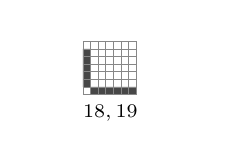
\begin{tikzpicture}[x=1mm,y=1mm,baseline=0mm]
\path[use as bounding box] (0,-.7) rectangle (21.5,11.9);
\begin{scope}[shift={(7.0,3.4)},x=0.97mm,y=0.97mm]
\fill[black!72] (0,5) rectangle (1,6) (0,4) rectangle (1,5) (0,3) rectangle (1,4) (0,2) rectangle (1,3) (0,1) rectangle (1,2) (1,0) rectangle (2,1) (2,0) rectangle (3,1) (3,0) rectangle (4,1) (4,0) rectangle (5,1) (5,0) rectangle (6,1) (6,0) rectangle (7,1);
\draw[black!47,line width=.16pt] (0,0)--(0,7) (0,0)--(7,0) (1,0)--(1,7) (0,1)--(7,1) (2,0)--(2,7) (0,2)--(7,2) (3,0)--(3,7) (0,3)--(7,3) (4,0)--(4,7) (0,4)--(7,4) (5,0)--(5,7) (0,5)--(7,5) (6,0)--(6,7) (0,6)--(7,6) (7,0)--(7,7) (0,7)--(7,7);
\end{scope}
\node[inner sep=0pt,font=\scriptsize] at (10.5,1.1) {$18,19$};
\end{tikzpicture} &
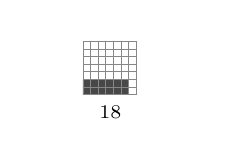
\begin{tikzpicture}[x=1mm,y=1mm,baseline=0mm]
\path[use as bounding box] (0,-.7) rectangle (21.5,11.9);
\begin{scope}[shift={(7.0,3.4)},x=0.97mm,y=0.97mm]
\fill[black!72] (0,1) rectangle (1,2) (1,1) rectangle (2,2) (2,1) rectangle (3,2) (3,1) rectangle (4,2) (4,1) rectangle (5,2) (5,1) rectangle (6,2) (0,0) rectangle (1,1) (1,0) rectangle (2,1) (2,0) rectangle (3,1) (3,0) rectangle (4,1) (4,0) rectangle (5,1) (5,0) rectangle (6,1);
\draw[black!47,line width=.16pt] (0,0)--(0,7) (0,0)--(7,0) (1,0)--(1,7) (0,1)--(7,1) (2,0)--(2,7) (0,2)--(7,2) (3,0)--(3,7) (0,3)--(7,3) (4,0)--(4,7) (0,4)--(7,4) (5,0)--(5,7) (0,5)--(7,5) (6,0)--(6,7) (0,6)--(7,6) (7,0)--(7,7) (0,7)--(7,7);
\end{scope}
\node[inner sep=0pt,font=\scriptsize] at (10.5,1.1) {$18$};
\end{tikzpicture} &
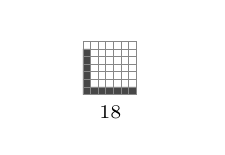
\begin{tikzpicture}[x=1mm,y=1mm,baseline=0mm]
\path[use as bounding box] (0,-.7) rectangle (21.5,11.9);
\begin{scope}[shift={(7.0,3.4)},x=0.97mm,y=0.97mm]
\fill[black!72] (0,5) rectangle (1,6) (0,4) rectangle (1,5) (0,3) rectangle (1,4) (0,2) rectangle (1,3) (0,1) rectangle (1,2) (0,0) rectangle (1,1) (1,0) rectangle (2,1) (2,0) rectangle (3,1) (3,0) rectangle (4,1) (4,0) rectangle (5,1) (5,0) rectangle (6,1) (6,0) rectangle (7,1);
\draw[black!47,line width=.16pt] (0,0)--(0,7) (0,0)--(7,0) (1,0)--(1,7) (0,1)--(7,1) (2,0)--(2,7) (0,2)--(7,2) (3,0)--(3,7) (0,3)--(7,3) (4,0)--(4,7) (0,4)--(7,4) (5,0)--(5,7) (0,5)--(7,5) (6,0)--(6,7) (0,6)--(7,6) (7,0)--(7,7) (0,7)--(7,7);
\end{scope}
\node[inner sep=0pt,font=\scriptsize] at (10.5,1.1) {$18$};
\end{tikzpicture} &
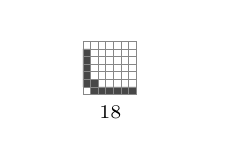
\begin{tikzpicture}[x=1mm,y=1mm,baseline=0mm]
\path[use as bounding box] (0,-.7) rectangle (21.5,11.9);
\begin{scope}[shift={(7.0,3.4)},x=0.97mm,y=0.97mm]
\fill[black!72] (0,5) rectangle (1,6) (0,4) rectangle (1,5) (0,3) rectangle (1,4) (0,2) rectangle (1,3) (0,1) rectangle (1,2) (1,1) rectangle (2,2) (1,0) rectangle (2,1) (2,0) rectangle (3,1) (3,0) rectangle (4,1) (4,0) rectangle (5,1) (5,0) rectangle (6,1) (6,0) rectangle (7,1);
\draw[black!47,line width=.16pt] (0,0)--(0,7) (0,0)--(7,0) (1,0)--(1,7) (0,1)--(7,1) (2,0)--(2,7) (0,2)--(7,2) (3,0)--(3,7) (0,3)--(7,3) (4,0)--(4,7) (0,4)--(7,4) (5,0)--(5,7) (0,5)--(7,5) (6,0)--(6,7) (0,6)--(7,6) (7,0)--(7,7) (0,7)--(7,7);
\end{scope}
\node[inner sep=0pt,font=\scriptsize] at (10.5,1.1) {$18$};
\end{tikzpicture} &
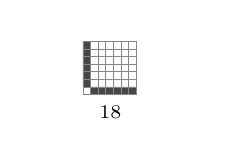
\begin{tikzpicture}[x=1mm,y=1mm,baseline=0mm]
\path[use as bounding box] (0,-.7) rectangle (21.5,11.9);
\begin{scope}[shift={(7.0,3.4)},x=0.97mm,y=0.97mm]
\fill[black!72] (0,6) rectangle (1,7) (0,5) rectangle (1,6) (0,4) rectangle (1,5) (0,3) rectangle (1,4) (0,2) rectangle (1,3) (0,1) rectangle (1,2) (1,0) rectangle (2,1) (2,0) rectangle (3,1) (3,0) rectangle (4,1) (4,0) rectangle (5,1) (5,0) rectangle (6,1) (6,0) rectangle (7,1);
\draw[black!47,line width=.16pt] (0,0)--(0,7) (0,0)--(7,0) (1,0)--(1,7) (0,1)--(7,1) (2,0)--(2,7) (0,2)--(7,2) (3,0)--(3,7) (0,3)--(7,3) (4,0)--(4,7) (0,4)--(7,4) (5,0)--(5,7) (0,5)--(7,5) (6,0)--(6,7) (0,6)--(7,6) (7,0)--(7,7) (0,7)--(7,7);
\end{scope}
\node[inner sep=0pt,font=\scriptsize] at (10.5,1.1) {$18$};
\end{tikzpicture} \\[.4mm]
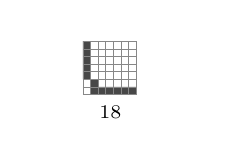
\begin{tikzpicture}[x=1mm,y=1mm,baseline=0mm]
\path[use as bounding box] (0,-.7) rectangle (21.5,11.9);
\begin{scope}[shift={(7.0,3.4)},x=0.97mm,y=0.97mm]
\fill[black!72] (0,6) rectangle (1,7) (0,5) rectangle (1,6) (0,4) rectangle (1,5) (0,3) rectangle (1,4) (0,2) rectangle (1,3) (1,1) rectangle (2,2) (1,0) rectangle (2,1) (2,0) rectangle (3,1) (3,0) rectangle (4,1) (4,0) rectangle (5,1) (5,0) rectangle (6,1) (6,0) rectangle (7,1);
\draw[black!47,line width=.16pt] (0,0)--(0,7) (0,0)--(7,0) (1,0)--(1,7) (0,1)--(7,1) (2,0)--(2,7) (0,2)--(7,2) (3,0)--(3,7) (0,3)--(7,3) (4,0)--(4,7) (0,4)--(7,4) (5,0)--(5,7) (0,5)--(7,5) (6,0)--(6,7) (0,6)--(7,6) (7,0)--(7,7) (0,7)--(7,7);
\end{scope}
\node[inner sep=0pt,font=\scriptsize] at (10.5,1.1) {$18$};
\end{tikzpicture} &
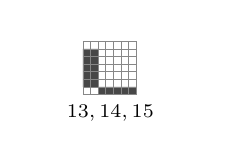
\begin{tikzpicture}[x=1mm,y=1mm,baseline=0mm]
\path[use as bounding box] (0,-.7) rectangle (21.5,11.9);
\begin{scope}[shift={(7.0,3.4)},x=0.97mm,y=0.97mm]
\fill[black!72] (0,5) rectangle (1,6) (1,5) rectangle (2,6) (0,4) rectangle (1,5) (1,4) rectangle (2,5) (0,3) rectangle (1,4) (1,3) rectangle (2,4) (0,2) rectangle (1,3) (1,2) rectangle (2,3) (0,1) rectangle (1,2) (1,1) rectangle (2,2) (2,0) rectangle (3,1) (3,0) rectangle (4,1) (4,0) rectangle (5,1) (5,0) rectangle (6,1) (6,0) rectangle (7,1);
\draw[black!47,line width=.16pt] (0,0)--(0,7) (0,0)--(7,0) (1,0)--(1,7) (0,1)--(7,1) (2,0)--(2,7) (0,2)--(7,2) (3,0)--(3,7) (0,3)--(7,3) (4,0)--(4,7) (0,4)--(7,4) (5,0)--(5,7) (0,5)--(7,5) (6,0)--(6,7) (0,6)--(7,6) (7,0)--(7,7) (0,7)--(7,7);
\end{scope}
\node[inner sep=0pt,font=\scriptsize] at (10.5,1.1) {$13,14,15$};
\end{tikzpicture} &
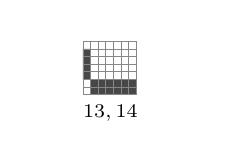
\begin{tikzpicture}[x=1mm,y=1mm,baseline=0mm]
\path[use as bounding box] (0,-.7) rectangle (21.5,11.9);
\begin{scope}[shift={(7.0,3.4)},x=0.97mm,y=0.97mm]
\fill[black!72] (0,5) rectangle (1,6) (0,4) rectangle (1,5) (0,3) rectangle (1,4) (0,2) rectangle (1,3) (1,1) rectangle (2,2) (2,1) rectangle (3,2) (3,1) rectangle (4,2) (4,1) rectangle (5,2) (5,1) rectangle (6,2) (6,1) rectangle (7,2) (1,0) rectangle (2,1) (2,0) rectangle (3,1) (3,0) rectangle (4,1) (4,0) rectangle (5,1) (5,0) rectangle (6,1) (6,0) rectangle (7,1);
\draw[black!47,line width=.16pt] (0,0)--(0,7) (0,0)--(7,0) (1,0)--(1,7) (0,1)--(7,1) (2,0)--(2,7) (0,2)--(7,2) (3,0)--(3,7) (0,3)--(7,3) (4,0)--(4,7) (0,4)--(7,4) (5,0)--(5,7) (0,5)--(7,5) (6,0)--(6,7) (0,6)--(7,6) (7,0)--(7,7) (0,7)--(7,7);
\end{scope}
\node[inner sep=0pt,font=\scriptsize] at (10.5,1.1) {$13,14$};
\end{tikzpicture} &
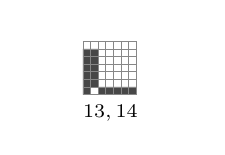
\begin{tikzpicture}[x=1mm,y=1mm,baseline=0mm]
\path[use as bounding box] (0,-.7) rectangle (21.5,11.9);
\begin{scope}[shift={(7.0,3.4)},x=0.97mm,y=0.97mm]
\fill[black!72] (0,5) rectangle (1,6) (1,5) rectangle (2,6) (0,4) rectangle (1,5) (1,4) rectangle (2,5) (0,3) rectangle (1,4) (1,3) rectangle (2,4) (0,2) rectangle (1,3) (1,2) rectangle (2,3) (0,1) rectangle (1,2) (1,1) rectangle (2,2) (0,0) rectangle (1,1) (2,0) rectangle (3,1) (3,0) rectangle (4,1) (4,0) rectangle (5,1) (5,0) rectangle (6,1) (6,0) rectangle (7,1);
\draw[black!47,line width=.16pt] (0,0)--(0,7) (0,0)--(7,0) (1,0)--(1,7) (0,1)--(7,1) (2,0)--(2,7) (0,2)--(7,2) (3,0)--(3,7) (0,3)--(7,3) (4,0)--(4,7) (0,4)--(7,4) (5,0)--(5,7) (0,5)--(7,5) (6,0)--(6,7) (0,6)--(7,6) (7,0)--(7,7) (0,7)--(7,7);
\end{scope}
\node[inner sep=0pt,font=\scriptsize] at (10.5,1.1) {$13,14$};
\end{tikzpicture} &
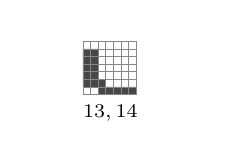
\begin{tikzpicture}[x=1mm,y=1mm,baseline=0mm]
\path[use as bounding box] (0,-.7) rectangle (21.5,11.9);
\begin{scope}[shift={(7.0,3.4)},x=0.97mm,y=0.97mm]
\fill[black!72] (0,5) rectangle (1,6) (1,5) rectangle (2,6) (0,4) rectangle (1,5) (1,4) rectangle (2,5) (0,3) rectangle (1,4) (1,3) rectangle (2,4) (0,2) rectangle (1,3) (1,2) rectangle (2,3) (0,1) rectangle (1,2) (1,1) rectangle (2,2) (2,1) rectangle (3,2) (2,0) rectangle (3,1) (3,0) rectangle (4,1) (4,0) rectangle (5,1) (5,0) rectangle (6,1) (6,0) rectangle (7,1);
\draw[black!47,line width=.16pt] (0,0)--(0,7) (0,0)--(7,0) (1,0)--(1,7) (0,1)--(7,1) (2,0)--(2,7) (0,2)--(7,2) (3,0)--(3,7) (0,3)--(7,3) (4,0)--(4,7) (0,4)--(7,4) (5,0)--(5,7) (0,5)--(7,5) (6,0)--(6,7) (0,6)--(7,6) (7,0)--(7,7) (0,7)--(7,7);
\end{scope}
\node[inner sep=0pt,font=\scriptsize] at (10.5,1.1) {$13,14$};
\end{tikzpicture} \\[.4mm]
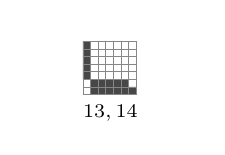
\begin{tikzpicture}[x=1mm,y=1mm,baseline=0mm]
\path[use as bounding box] (0,-.7) rectangle (21.5,11.9);
\begin{scope}[shift={(7.0,3.4)},x=0.97mm,y=0.97mm]
\fill[black!72] (0,6) rectangle (1,7) (0,5) rectangle (1,6) (0,4) rectangle (1,5) (0,3) rectangle (1,4) (0,2) rectangle (1,3) (1,1) rectangle (2,2) (2,1) rectangle (3,2) (3,1) rectangle (4,2) (4,1) rectangle (5,2) (5,1) rectangle (6,2) (1,0) rectangle (2,1) (2,0) rectangle (3,1) (3,0) rectangle (4,1) (4,0) rectangle (5,1) (5,0) rectangle (6,1) (6,0) rectangle (7,1);
\draw[black!47,line width=.16pt] (0,0)--(0,7) (0,0)--(7,0) (1,0)--(1,7) (0,1)--(7,1) (2,0)--(2,7) (0,2)--(7,2) (3,0)--(3,7) (0,3)--(7,3) (4,0)--(4,7) (0,4)--(7,4) (5,0)--(5,7) (0,5)--(7,5) (6,0)--(6,7) (0,6)--(7,6) (7,0)--(7,7) (0,7)--(7,7);
\end{scope}
\node[inner sep=0pt,font=\scriptsize] at (10.5,1.1) {$13,14$};
\end{tikzpicture} &
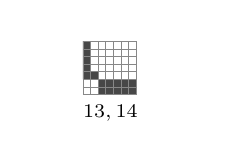
\begin{tikzpicture}[x=1mm,y=1mm,baseline=0mm]
\path[use as bounding box] (0,-.7) rectangle (21.5,11.9);
\begin{scope}[shift={(7.0,3.4)},x=0.97mm,y=0.97mm]
\fill[black!72] (0,6) rectangle (1,7) (0,5) rectangle (1,6) (0,4) rectangle (1,5) (0,3) rectangle (1,4) (0,2) rectangle (1,3) (1,2) rectangle (2,3) (2,1) rectangle (3,2) (3,1) rectangle (4,2) (4,1) rectangle (5,2) (5,1) rectangle (6,2) (6,1) rectangle (7,2) (2,0) rectangle (3,1) (3,0) rectangle (4,1) (4,0) rectangle (5,1) (5,0) rectangle (6,1) (6,0) rectangle (7,1);
\draw[black!47,line width=.16pt] (0,0)--(0,7) (0,0)--(7,0) (1,0)--(1,7) (0,1)--(7,1) (2,0)--(2,7) (0,2)--(7,2) (3,0)--(3,7) (0,3)--(7,3) (4,0)--(4,7) (0,4)--(7,4) (5,0)--(5,7) (0,5)--(7,5) (6,0)--(6,7) (0,6)--(7,6) (7,0)--(7,7) (0,7)--(7,7);
\end{scope}
\node[inner sep=0pt,font=\scriptsize] at (10.5,1.1) {$13,14$};
\end{tikzpicture} &
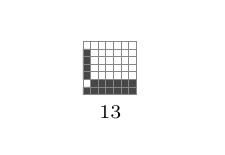
\begin{tikzpicture}[x=1mm,y=1mm,baseline=0mm]
\path[use as bounding box] (0,-.7) rectangle (21.5,11.9);
\begin{scope}[shift={(7.0,3.4)},x=0.97mm,y=0.97mm]
\fill[black!72] (0,5) rectangle (1,6) (0,4) rectangle (1,5) (0,3) rectangle (1,4) (0,2) rectangle (1,3) (1,1) rectangle (2,2) (2,1) rectangle (3,2) (3,1) rectangle (4,2) (4,1) rectangle (5,2) (5,1) rectangle (6,2) (6,1) rectangle (7,2) (0,0) rectangle (1,1) (1,0) rectangle (2,1) (2,0) rectangle (3,1) (3,0) rectangle (4,1) (4,0) rectangle (5,1) (5,0) rectangle (6,1) (6,0) rectangle (7,1);
\draw[black!47,line width=.16pt] (0,0)--(0,7) (0,0)--(7,0) (1,0)--(1,7) (0,1)--(7,1) (2,0)--(2,7) (0,2)--(7,2) (3,0)--(3,7) (0,3)--(7,3) (4,0)--(4,7) (0,4)--(7,4) (5,0)--(5,7) (0,5)--(7,5) (6,0)--(6,7) (0,6)--(7,6) (7,0)--(7,7) (0,7)--(7,7);
\end{scope}
\node[inner sep=0pt,font=\scriptsize] at (10.5,1.1) {$13$};
\end{tikzpicture} &
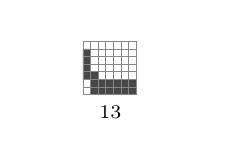
\begin{tikzpicture}[x=1mm,y=1mm,baseline=0mm]
\path[use as bounding box] (0,-.7) rectangle (21.5,11.9);
\begin{scope}[shift={(7.0,3.4)},x=0.97mm,y=0.97mm]
\fill[black!72] (0,5) rectangle (1,6) (0,4) rectangle (1,5) (0,3) rectangle (1,4) (0,2) rectangle (1,3) (1,2) rectangle (2,3) (1,1) rectangle (2,2) (2,1) rectangle (3,2) (3,1) rectangle (4,2) (4,1) rectangle (5,2) (5,1) rectangle (6,2) (6,1) rectangle (7,2) (1,0) rectangle (2,1) (2,0) rectangle (3,1) (3,0) rectangle (4,1) (4,0) rectangle (5,1) (5,0) rectangle (6,1) (6,0) rectangle (7,1);
\draw[black!47,line width=.16pt] (0,0)--(0,7) (0,0)--(7,0) (1,0)--(1,7) (0,1)--(7,1) (2,0)--(2,7) (0,2)--(7,2) (3,0)--(3,7) (0,3)--(7,3) (4,0)--(4,7) (0,4)--(7,4) (5,0)--(5,7) (0,5)--(7,5) (6,0)--(6,7) (0,6)--(7,6) (7,0)--(7,7) (0,7)--(7,7);
\end{scope}
\node[inner sep=0pt,font=\scriptsize] at (10.5,1.1) {$13$};
\end{tikzpicture} &
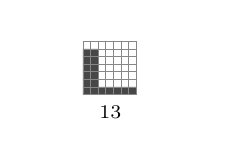
\begin{tikzpicture}[x=1mm,y=1mm,baseline=0mm]
\path[use as bounding box] (0,-.7) rectangle (21.5,11.9);
\begin{scope}[shift={(7.0,3.4)},x=0.97mm,y=0.97mm]
\fill[black!72] (0,5) rectangle (1,6) (1,5) rectangle (2,6) (0,4) rectangle (1,5) (1,4) rectangle (2,5) (0,3) rectangle (1,4) (1,3) rectangle (2,4) (0,2) rectangle (1,3) (1,2) rectangle (2,3) (0,1) rectangle (1,2) (1,1) rectangle (2,2) (0,0) rectangle (1,1) (1,0) rectangle (2,1) (2,0) rectangle (3,1) (3,0) rectangle (4,1) (4,0) rectangle (5,1) (5,0) rectangle (6,1) (6,0) rectangle (7,1);
\draw[black!47,line width=.16pt] (0,0)--(0,7) (0,0)--(7,0) (1,0)--(1,7) (0,1)--(7,1) (2,0)--(2,7) (0,2)--(7,2) (3,0)--(3,7) (0,3)--(7,3) (4,0)--(4,7) (0,4)--(7,4) (5,0)--(5,7) (0,5)--(7,5) (6,0)--(6,7) (0,6)--(7,6) (7,0)--(7,7) (0,7)--(7,7);
\end{scope}
\node[inner sep=0pt,font=\scriptsize] at (10.5,1.1) {$13$};
\end{tikzpicture} \\[.4mm]
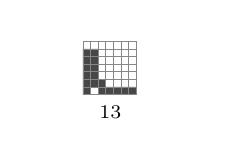
\begin{tikzpicture}[x=1mm,y=1mm,baseline=0mm]
\path[use as bounding box] (0,-.7) rectangle (21.5,11.9);
\begin{scope}[shift={(7.0,3.4)},x=0.97mm,y=0.97mm]
\fill[black!72] (0,5) rectangle (1,6) (1,5) rectangle (2,6) (0,4) rectangle (1,5) (1,4) rectangle (2,5) (0,3) rectangle (1,4) (1,3) rectangle (2,4) (0,2) rectangle (1,3) (1,2) rectangle (2,3) (0,1) rectangle (1,2) (1,1) rectangle (2,2) (2,1) rectangle (3,2) (0,0) rectangle (1,1) (2,0) rectangle (3,1) (3,0) rectangle (4,1) (4,0) rectangle (5,1) (5,0) rectangle (6,1) (6,0) rectangle (7,1);
\draw[black!47,line width=.16pt] (0,0)--(0,7) (0,0)--(7,0) (1,0)--(1,7) (0,1)--(7,1) (2,0)--(2,7) (0,2)--(7,2) (3,0)--(3,7) (0,3)--(7,3) (4,0)--(4,7) (0,4)--(7,4) (5,0)--(5,7) (0,5)--(7,5) (6,0)--(6,7) (0,6)--(7,6) (7,0)--(7,7) (0,7)--(7,7);
\end{scope}
\node[inner sep=0pt,font=\scriptsize] at (10.5,1.1) {$13$};
\end{tikzpicture} &
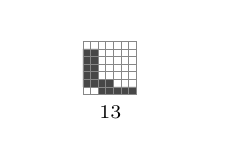
\begin{tikzpicture}[x=1mm,y=1mm,baseline=0mm]
\path[use as bounding box] (0,-.7) rectangle (21.5,11.9);
\begin{scope}[shift={(7.0,3.4)},x=0.97mm,y=0.97mm]
\fill[black!72] (0,5) rectangle (1,6) (1,5) rectangle (2,6) (0,4) rectangle (1,5) (1,4) rectangle (2,5) (0,3) rectangle (1,4) (1,3) rectangle (2,4) (0,2) rectangle (1,3) (1,2) rectangle (2,3) (0,1) rectangle (1,2) (1,1) rectangle (2,2) (2,1) rectangle (3,2) (3,1) rectangle (4,2) (2,0) rectangle (3,1) (3,0) rectangle (4,1) (4,0) rectangle (5,1) (5,0) rectangle (6,1) (6,0) rectangle (7,1);
\draw[black!47,line width=.16pt] (0,0)--(0,7) (0,0)--(7,0) (1,0)--(1,7) (0,1)--(7,1) (2,0)--(2,7) (0,2)--(7,2) (3,0)--(3,7) (0,3)--(7,3) (4,0)--(4,7) (0,4)--(7,4) (5,0)--(5,7) (0,5)--(7,5) (6,0)--(6,7) (0,6)--(7,6) (7,0)--(7,7) (0,7)--(7,7);
\end{scope}
\node[inner sep=0pt,font=\scriptsize] at (10.5,1.1) {$13$};
\end{tikzpicture} &
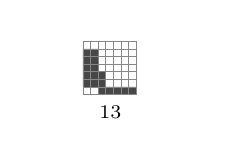
\begin{tikzpicture}[x=1mm,y=1mm,baseline=0mm]
\path[use as bounding box] (0,-.7) rectangle (21.5,11.9);
\begin{scope}[shift={(7.0,3.4)},x=0.97mm,y=0.97mm]
\fill[black!72] (0,5) rectangle (1,6) (1,5) rectangle (2,6) (0,4) rectangle (1,5) (1,4) rectangle (2,5) (0,3) rectangle (1,4) (1,3) rectangle (2,4) (0,2) rectangle (1,3) (1,2) rectangle (2,3) (2,2) rectangle (3,3) (0,1) rectangle (1,2) (1,1) rectangle (2,2) (2,1) rectangle (3,2) (2,0) rectangle (3,1) (3,0) rectangle (4,1) (4,0) rectangle (5,1) (5,0) rectangle (6,1) (6,0) rectangle (7,1);
\draw[black!47,line width=.16pt] (0,0)--(0,7) (0,0)--(7,0) (1,0)--(1,7) (0,1)--(7,1) (2,0)--(2,7) (0,2)--(7,2) (3,0)--(3,7) (0,3)--(7,3) (4,0)--(4,7) (0,4)--(7,4) (5,0)--(5,7) (0,5)--(7,5) (6,0)--(6,7) (0,6)--(7,6) (7,0)--(7,7) (0,7)--(7,7);
\end{scope}
\node[inner sep=0pt,font=\scriptsize] at (10.5,1.1) {$13$};
\end{tikzpicture} &
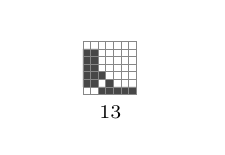
\begin{tikzpicture}[x=1mm,y=1mm,baseline=0mm]
\path[use as bounding box] (0,-.7) rectangle (21.5,11.9);
\begin{scope}[shift={(7.0,3.4)},x=0.97mm,y=0.97mm]
\fill[black!72] (0,5) rectangle (1,6) (1,5) rectangle (2,6) (0,4) rectangle (1,5) (1,4) rectangle (2,5) (0,3) rectangle (1,4) (1,3) rectangle (2,4) (0,2) rectangle (1,3) (1,2) rectangle (2,3) (2,2) rectangle (3,3) (0,1) rectangle (1,2) (1,1) rectangle (2,2) (3,1) rectangle (4,2) (2,0) rectangle (3,1) (3,0) rectangle (4,1) (4,0) rectangle (5,1) (5,0) rectangle (6,1) (6,0) rectangle (7,1);
\draw[black!47,line width=.16pt] (0,0)--(0,7) (0,0)--(7,0) (1,0)--(1,7) (0,1)--(7,1) (2,0)--(2,7) (0,2)--(7,2) (3,0)--(3,7) (0,3)--(7,3) (4,0)--(4,7) (0,4)--(7,4) (5,0)--(5,7) (0,5)--(7,5) (6,0)--(6,7) (0,6)--(7,6) (7,0)--(7,7) (0,7)--(7,7);
\end{scope}
\node[inner sep=0pt,font=\scriptsize] at (10.5,1.1) {$13$};
\end{tikzpicture} &
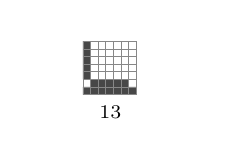
\begin{tikzpicture}[x=1mm,y=1mm,baseline=0mm]
\path[use as bounding box] (0,-.7) rectangle (21.5,11.9);
\begin{scope}[shift={(7.0,3.4)},x=0.97mm,y=0.97mm]
\fill[black!72] (0,6) rectangle (1,7) (0,5) rectangle (1,6) (0,4) rectangle (1,5) (0,3) rectangle (1,4) (0,2) rectangle (1,3) (1,1) rectangle (2,2) (2,1) rectangle (3,2) (3,1) rectangle (4,2) (4,1) rectangle (5,2) (5,1) rectangle (6,2) (0,0) rectangle (1,1) (1,0) rectangle (2,1) (2,0) rectangle (3,1) (3,0) rectangle (4,1) (4,0) rectangle (5,1) (5,0) rectangle (6,1) (6,0) rectangle (7,1);
\draw[black!47,line width=.16pt] (0,0)--(0,7) (0,0)--(7,0) (1,0)--(1,7) (0,1)--(7,1) (2,0)--(2,7) (0,2)--(7,2) (3,0)--(3,7) (0,3)--(7,3) (4,0)--(4,7) (0,4)--(7,4) (5,0)--(5,7) (0,5)--(7,5) (6,0)--(6,7) (0,6)--(7,6) (7,0)--(7,7) (0,7)--(7,7);
\end{scope}
\node[inner sep=0pt,font=\scriptsize] at (10.5,1.1) {$13$};
\end{tikzpicture} \\[.4mm]
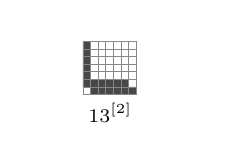
\begin{tikzpicture}[x=1mm,y=1mm,baseline=0mm]
\path[use as bounding box] (0,-.7) rectangle (21.5,11.9);
\begin{scope}[shift={(7.0,3.4)},x=0.97mm,y=0.97mm]
\fill[black!72] (0,6) rectangle (1,7) (0,5) rectangle (1,6) (0,4) rectangle (1,5) (0,3) rectangle (1,4) (0,2) rectangle (1,3) (0,1) rectangle (1,2) (1,1) rectangle (2,2) (2,1) rectangle (3,2) (3,1) rectangle (4,2) (4,1) rectangle (5,2) (5,1) rectangle (6,2) (1,0) rectangle (2,1) (2,0) rectangle (3,1) (3,0) rectangle (4,1) (4,0) rectangle (5,1) (5,0) rectangle (6,1) (6,0) rectangle (7,1);
\draw[black!47,line width=.16pt] (0,0)--(0,7) (0,0)--(7,0) (1,0)--(1,7) (0,1)--(7,1) (2,0)--(2,7) (0,2)--(7,2) (3,0)--(3,7) (0,3)--(7,3) (4,0)--(4,7) (0,4)--(7,4) (5,0)--(5,7) (0,5)--(7,5) (6,0)--(6,7) (0,6)--(7,6) (7,0)--(7,7) (0,7)--(7,7);
\end{scope}
\node[inner sep=0pt,font=\scriptsize] at (10.5,1.1) {$13^{[2]}$};
\end{tikzpicture} &
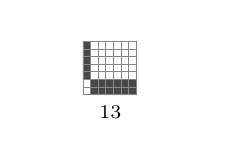
\begin{tikzpicture}[x=1mm,y=1mm,baseline=0mm]
\path[use as bounding box] (0,-.7) rectangle (21.5,11.9);
\begin{scope}[shift={(7.0,3.4)},x=0.97mm,y=0.97mm]
\fill[black!72] (0,6) rectangle (1,7) (0,5) rectangle (1,6) (0,4) rectangle (1,5) (0,3) rectangle (1,4) (0,2) rectangle (1,3) (1,1) rectangle (2,2) (2,1) rectangle (3,2) (3,1) rectangle (4,2) (4,1) rectangle (5,2) (5,1) rectangle (6,2) (6,1) rectangle (7,2) (1,0) rectangle (2,1) (2,0) rectangle (3,1) (3,0) rectangle (4,1) (4,0) rectangle (5,1) (5,0) rectangle (6,1) (6,0) rectangle (7,1);
\draw[black!47,line width=.16pt] (0,0)--(0,7) (0,0)--(7,0) (1,0)--(1,7) (0,1)--(7,1) (2,0)--(2,7) (0,2)--(7,2) (3,0)--(3,7) (0,3)--(7,3) (4,0)--(4,7) (0,4)--(7,4) (5,0)--(5,7) (0,5)--(7,5) (6,0)--(6,7) (0,6)--(7,6) (7,0)--(7,7) (0,7)--(7,7);
\end{scope}
\node[inner sep=0pt,font=\scriptsize] at (10.5,1.1) {$13$};
\end{tikzpicture} &
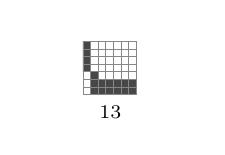
\begin{tikzpicture}[x=1mm,y=1mm,baseline=0mm]
\path[use as bounding box] (0,-.7) rectangle (21.5,11.9);
\begin{scope}[shift={(7.0,3.4)},x=0.97mm,y=0.97mm]
\fill[black!72] (0,6) rectangle (1,7) (0,5) rectangle (1,6) (0,4) rectangle (1,5) (0,3) rectangle (1,4) (1,2) rectangle (2,3) (1,1) rectangle (2,2) (2,1) rectangle (3,2) (3,1) rectangle (4,2) (4,1) rectangle (5,2) (5,1) rectangle (6,2) (6,1) rectangle (7,2) (1,0) rectangle (2,1) (2,0) rectangle (3,1) (3,0) rectangle (4,1) (4,0) rectangle (5,1) (5,0) rectangle (6,1) (6,0) rectangle (7,1);
\draw[black!47,line width=.16pt] (0,0)--(0,7) (0,0)--(7,0) (1,0)--(1,7) (0,1)--(7,1) (2,0)--(2,7) (0,2)--(7,2) (3,0)--(3,7) (0,3)--(7,3) (4,0)--(4,7) (0,4)--(7,4) (5,0)--(5,7) (0,5)--(7,5) (6,0)--(6,7) (0,6)--(7,6) (7,0)--(7,7) (0,7)--(7,7);
\end{scope}
\node[inner sep=0pt,font=\scriptsize] at (10.5,1.1) {$13$};
\end{tikzpicture} &
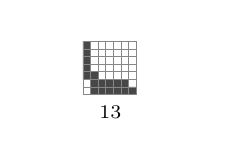
\begin{tikzpicture}[x=1mm,y=1mm,baseline=0mm]
\path[use as bounding box] (0,-.7) rectangle (21.5,11.9);
\begin{scope}[shift={(7.0,3.4)},x=0.97mm,y=0.97mm]
\fill[black!72] (0,6) rectangle (1,7) (0,5) rectangle (1,6) (0,4) rectangle (1,5) (0,3) rectangle (1,4) (0,2) rectangle (1,3) (1,2) rectangle (2,3) (1,1) rectangle (2,2) (2,1) rectangle (3,2) (3,1) rectangle (4,2) (4,1) rectangle (5,2) (5,1) rectangle (6,2) (1,0) rectangle (2,1) (2,0) rectangle (3,1) (3,0) rectangle (4,1) (4,0) rectangle (5,1) (5,0) rectangle (6,1) (6,0) rectangle (7,1);
\draw[black!47,line width=.16pt] (0,0)--(0,7) (0,0)--(7,0) (1,0)--(1,7) (0,1)--(7,1) (2,0)--(2,7) (0,2)--(7,2) (3,0)--(3,7) (0,3)--(7,3) (4,0)--(4,7) (0,4)--(7,4) (5,0)--(5,7) (0,5)--(7,5) (6,0)--(6,7) (0,6)--(7,6) (7,0)--(7,7) (0,7)--(7,7);
\end{scope}
\node[inner sep=0pt,font=\scriptsize] at (10.5,1.1) {$13$};
\end{tikzpicture} &
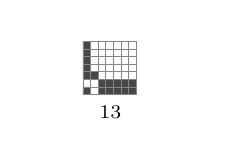
\begin{tikzpicture}[x=1mm,y=1mm,baseline=0mm]
\path[use as bounding box] (0,-.7) rectangle (21.5,11.9);
\begin{scope}[shift={(7.0,3.4)},x=0.97mm,y=0.97mm]
\fill[black!72] (0,6) rectangle (1,7) (0,5) rectangle (1,6) (0,4) rectangle (1,5) (0,3) rectangle (1,4) (0,2) rectangle (1,3) (1,2) rectangle (2,3) (2,1) rectangle (3,2) (3,1) rectangle (4,2) (4,1) rectangle (5,2) (5,1) rectangle (6,2) (6,1) rectangle (7,2) (0,0) rectangle (1,1) (2,0) rectangle (3,1) (3,0) rectangle (4,1) (4,0) rectangle (5,1) (5,0) rectangle (6,1) (6,0) rectangle (7,1);
\draw[black!47,line width=.16pt] (0,0)--(0,7) (0,0)--(7,0) (1,0)--(1,7) (0,1)--(7,1) (2,0)--(2,7) (0,2)--(7,2) (3,0)--(3,7) (0,3)--(7,3) (4,0)--(4,7) (0,4)--(7,4) (5,0)--(5,7) (0,5)--(7,5) (6,0)--(6,7) (0,6)--(7,6) (7,0)--(7,7) (0,7)--(7,7);
\end{scope}
\node[inner sep=0pt,font=\scriptsize] at (10.5,1.1) {$13$};
\end{tikzpicture} \\[.4mm]
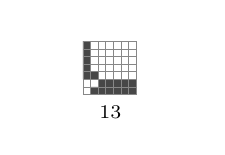
\begin{tikzpicture}[x=1mm,y=1mm,baseline=0mm]
\path[use as bounding box] (0,-.7) rectangle (21.5,11.9);
\begin{scope}[shift={(7.0,3.4)},x=0.97mm,y=0.97mm]
\fill[black!72] (0,6) rectangle (1,7) (0,5) rectangle (1,6) (0,4) rectangle (1,5) (0,3) rectangle (1,4) (0,2) rectangle (1,3) (1,2) rectangle (2,3) (2,1) rectangle (3,2) (3,1) rectangle (4,2) (4,1) rectangle (5,2) (5,1) rectangle (6,2) (6,1) rectangle (7,2) (1,0) rectangle (2,1) (2,0) rectangle (3,1) (3,0) rectangle (4,1) (4,0) rectangle (5,1) (5,0) rectangle (6,1) (6,0) rectangle (7,1);
\draw[black!47,line width=.16pt] (0,0)--(0,7) (0,0)--(7,0) (1,0)--(1,7) (0,1)--(7,1) (2,0)--(2,7) (0,2)--(7,2) (3,0)--(3,7) (0,3)--(7,3) (4,0)--(4,7) (0,4)--(7,4) (5,0)--(5,7) (0,5)--(7,5) (6,0)--(6,7) (0,6)--(7,6) (7,0)--(7,7) (0,7)--(7,7);
\end{scope}
\node[inner sep=0pt,font=\scriptsize] at (10.5,1.1) {$13$};
\end{tikzpicture} &
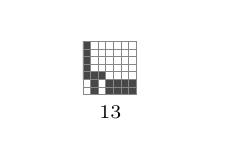
\begin{tikzpicture}[x=1mm,y=1mm,baseline=0mm]
\path[use as bounding box] (0,-.7) rectangle (21.5,11.9);
\begin{scope}[shift={(7.0,3.4)},x=0.97mm,y=0.97mm]
\fill[black!72] (0,6) rectangle (1,7) (0,5) rectangle (1,6) (0,4) rectangle (1,5) (0,3) rectangle (1,4) (0,2) rectangle (1,3) (1,2) rectangle (2,3) (2,2) rectangle (3,3) (1,1) rectangle (2,2) (3,1) rectangle (4,2) (4,1) rectangle (5,2) (5,1) rectangle (6,2) (6,1) rectangle (7,2) (1,0) rectangle (2,1) (3,0) rectangle (4,1) (4,0) rectangle (5,1) (5,0) rectangle (6,1) (6,0) rectangle (7,1);
\draw[black!47,line width=.16pt] (0,0)--(0,7) (0,0)--(7,0) (1,0)--(1,7) (0,1)--(7,1) (2,0)--(2,7) (0,2)--(7,2) (3,0)--(3,7) (0,3)--(7,3) (4,0)--(4,7) (0,4)--(7,4) (5,0)--(5,7) (0,5)--(7,5) (6,0)--(6,7) (0,6)--(7,6) (7,0)--(7,7) (0,7)--(7,7);
\end{scope}
\node[inner sep=0pt,font=\scriptsize] at (10.5,1.1) {$13$};
\end{tikzpicture} &
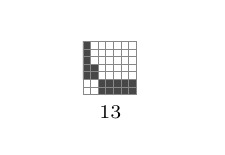
\begin{tikzpicture}[x=1mm,y=1mm,baseline=0mm]
\path[use as bounding box] (0,-.7) rectangle (21.5,11.9);
\begin{scope}[shift={(7.0,3.4)},x=0.97mm,y=0.97mm]
\fill[black!72] (0,6) rectangle (1,7) (0,5) rectangle (1,6) (0,4) rectangle (1,5) (0,3) rectangle (1,4) (1,3) rectangle (2,4) (0,2) rectangle (1,3) (1,2) rectangle (2,3) (2,1) rectangle (3,2) (3,1) rectangle (4,2) (4,1) rectangle (5,2) (5,1) rectangle (6,2) (6,1) rectangle (7,2) (2,0) rectangle (3,1) (3,0) rectangle (4,1) (4,0) rectangle (5,1) (5,0) rectangle (6,1) (6,0) rectangle (7,1);
\draw[black!47,line width=.16pt] (0,0)--(0,7) (0,0)--(7,0) (1,0)--(1,7) (0,1)--(7,1) (2,0)--(2,7) (0,2)--(7,2) (3,0)--(3,7) (0,3)--(7,3) (4,0)--(4,7) (0,4)--(7,4) (5,0)--(5,7) (0,5)--(7,5) (6,0)--(6,7) (0,6)--(7,6) (7,0)--(7,7) (0,7)--(7,7);
\end{scope}
\node[inner sep=0pt,font=\scriptsize] at (10.5,1.1) {$13$};
\end{tikzpicture} &
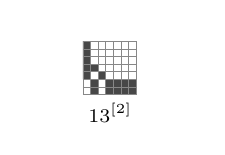
\begin{tikzpicture}[x=1mm,y=1mm,baseline=0mm]
\path[use as bounding box] (0,-.7) rectangle (21.5,11.9);
\begin{scope}[shift={(7.0,3.4)},x=0.97mm,y=0.97mm]
\fill[black!72] (0,6) rectangle (1,7) (0,5) rectangle (1,6) (0,4) rectangle (1,5) (0,3) rectangle (1,4) (1,3) rectangle (2,4) (0,2) rectangle (1,3) (2,2) rectangle (3,3) (1,1) rectangle (2,2) (3,1) rectangle (4,2) (4,1) rectangle (5,2) (5,1) rectangle (6,2) (6,1) rectangle (7,2) (1,0) rectangle (2,1) (3,0) rectangle (4,1) (4,0) rectangle (5,1) (5,0) rectangle (6,1) (6,0) rectangle (7,1);
\draw[black!47,line width=.16pt] (0,0)--(0,7) (0,0)--(7,0) (1,0)--(1,7) (0,1)--(7,1) (2,0)--(2,7) (0,2)--(7,2) (3,0)--(3,7) (0,3)--(7,3) (4,0)--(4,7) (0,4)--(7,4) (5,0)--(5,7) (0,5)--(7,5) (6,0)--(6,7) (0,6)--(7,6) (7,0)--(7,7) (0,7)--(7,7);
\end{scope}
\node[inner sep=0pt,font=\scriptsize] at (10.5,1.1) {$13^{[2]}$};
\end{tikzpicture} &
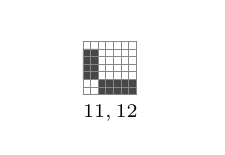
\begin{tikzpicture}[x=1mm,y=1mm,baseline=0mm]
\path[use as bounding box] (0,-.7) rectangle (21.5,11.9);
\begin{scope}[shift={(7.0,3.4)},x=0.97mm,y=0.97mm]
\fill[black!72] (0,5) rectangle (1,6) (1,5) rectangle (2,6) (0,4) rectangle (1,5) (1,4) rectangle (2,5) (0,3) rectangle (1,4) (1,3) rectangle (2,4) (0,2) rectangle (1,3) (1,2) rectangle (2,3) (2,1) rectangle (3,2) (3,1) rectangle (4,2) (4,1) rectangle (5,2) (5,1) rectangle (6,2) (6,1) rectangle (7,2) (2,0) rectangle (3,1) (3,0) rectangle (4,1) (4,0) rectangle (5,1) (5,0) rectangle (6,1) (6,0) rectangle (7,1);
\draw[black!47,line width=.16pt] (0,0)--(0,7) (0,0)--(7,0) (1,0)--(1,7) (0,1)--(7,1) (2,0)--(2,7) (0,2)--(7,2) (3,0)--(3,7) (0,3)--(7,3) (4,0)--(4,7) (0,4)--(7,4) (5,0)--(5,7) (0,5)--(7,5) (6,0)--(6,7) (0,6)--(7,6) (7,0)--(7,7) (0,7)--(7,7);
\end{scope}
\node[inner sep=0pt,font=\scriptsize] at (10.5,1.1) {$11,12$};
\end{tikzpicture} \\[.4mm]
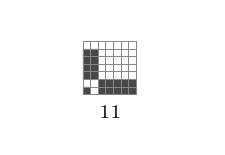
\begin{tikzpicture}[x=1mm,y=1mm,baseline=0mm]
\path[use as bounding box] (0,-.7) rectangle (21.5,11.9);
\begin{scope}[shift={(7.0,3.4)},x=0.97mm,y=0.97mm]
\fill[black!72] (0,5) rectangle (1,6) (1,5) rectangle (2,6) (0,4) rectangle (1,5) (1,4) rectangle (2,5) (0,3) rectangle (1,4) (1,3) rectangle (2,4) (0,2) rectangle (1,3) (1,2) rectangle (2,3) (2,1) rectangle (3,2) (3,1) rectangle (4,2) (4,1) rectangle (5,2) (5,1) rectangle (6,2) (6,1) rectangle (7,2) (0,0) rectangle (1,1) (2,0) rectangle (3,1) (3,0) rectangle (4,1) (4,0) rectangle (5,1) (5,0) rectangle (6,1) (6,0) rectangle (7,1);
\draw[black!47,line width=.16pt] (0,0)--(0,7) (0,0)--(7,0) (1,0)--(1,7) (0,1)--(7,1) (2,0)--(2,7) (0,2)--(7,2) (3,0)--(3,7) (0,3)--(7,3) (4,0)--(4,7) (0,4)--(7,4) (5,0)--(5,7) (0,5)--(7,5) (6,0)--(6,7) (0,6)--(7,6) (7,0)--(7,7) (0,7)--(7,7);
\end{scope}
\node[inner sep=0pt,font=\scriptsize] at (10.5,1.1) {$11$};
\end{tikzpicture} &
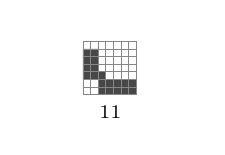
\begin{tikzpicture}[x=1mm,y=1mm,baseline=0mm]
\path[use as bounding box] (0,-.7) rectangle (21.5,11.9);
\begin{scope}[shift={(7.0,3.4)},x=0.97mm,y=0.97mm]
\fill[black!72] (0,5) rectangle (1,6) (1,5) rectangle (2,6) (0,4) rectangle (1,5) (1,4) rectangle (2,5) (0,3) rectangle (1,4) (1,3) rectangle (2,4) (0,2) rectangle (1,3) (1,2) rectangle (2,3) (2,2) rectangle (3,3) (2,1) rectangle (3,2) (3,1) rectangle (4,2) (4,1) rectangle (5,2) (5,1) rectangle (6,2) (6,1) rectangle (7,2) (2,0) rectangle (3,1) (3,0) rectangle (4,1) (4,0) rectangle (5,1) (5,0) rectangle (6,1) (6,0) rectangle (7,1);
\draw[black!47,line width=.16pt] (0,0)--(0,7) (0,0)--(7,0) (1,0)--(1,7) (0,1)--(7,1) (2,0)--(2,7) (0,2)--(7,2) (3,0)--(3,7) (0,3)--(7,3) (4,0)--(4,7) (0,4)--(7,4) (5,0)--(5,7) (0,5)--(7,5) (6,0)--(6,7) (0,6)--(7,6) (7,0)--(7,7) (0,7)--(7,7);
\end{scope}
\node[inner sep=0pt,font=\scriptsize] at (10.5,1.1) {$11$};
\end{tikzpicture} &
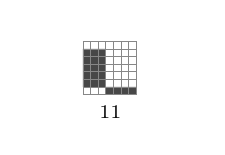
\begin{tikzpicture}[x=1mm,y=1mm,baseline=0mm]
\path[use as bounding box] (0,-.7) rectangle (21.5,11.9);
\begin{scope}[shift={(7.0,3.4)},x=0.97mm,y=0.97mm]
\fill[black!72] (0,5) rectangle (1,6) (1,5) rectangle (2,6) (2,5) rectangle (3,6) (0,4) rectangle (1,5) (1,4) rectangle (2,5) (2,4) rectangle (3,5) (0,3) rectangle (1,4) (1,3) rectangle (2,4) (2,3) rectangle (3,4) (0,2) rectangle (1,3) (1,2) rectangle (2,3) (2,2) rectangle (3,3) (0,1) rectangle (1,2) (1,1) rectangle (2,2) (2,1) rectangle (3,2) (3,0) rectangle (4,1) (4,0) rectangle (5,1) (5,0) rectangle (6,1) (6,0) rectangle (7,1);
\draw[black!47,line width=.16pt] (0,0)--(0,7) (0,0)--(7,0) (1,0)--(1,7) (0,1)--(7,1) (2,0)--(2,7) (0,2)--(7,2) (3,0)--(3,7) (0,3)--(7,3) (4,0)--(4,7) (0,4)--(7,4) (5,0)--(5,7) (0,5)--(7,5) (6,0)--(6,7) (0,6)--(7,6) (7,0)--(7,7) (0,7)--(7,7);
\end{scope}
\node[inner sep=0pt,font=\scriptsize] at (10.5,1.1) {$11$};
\end{tikzpicture} &
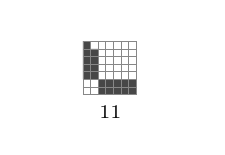
\begin{tikzpicture}[x=1mm,y=1mm,baseline=0mm]
\path[use as bounding box] (0,-.7) rectangle (21.5,11.9);
\begin{scope}[shift={(7.0,3.4)},x=0.97mm,y=0.97mm]
\fill[black!72] (0,6) rectangle (1,7) (0,5) rectangle (1,6) (1,5) rectangle (2,6) (0,4) rectangle (1,5) (1,4) rectangle (2,5) (0,3) rectangle (1,4) (1,3) rectangle (2,4) (0,2) rectangle (1,3) (1,2) rectangle (2,3) (2,1) rectangle (3,2) (3,1) rectangle (4,2) (4,1) rectangle (5,2) (5,1) rectangle (6,2) (6,1) rectangle (7,2) (2,0) rectangle (3,1) (3,0) rectangle (4,1) (4,0) rectangle (5,1) (5,0) rectangle (6,1) (6,0) rectangle (7,1);
\draw[black!47,line width=.16pt] (0,0)--(0,7) (0,0)--(7,0) (1,0)--(1,7) (0,1)--(7,1) (2,0)--(2,7) (0,2)--(7,2) (3,0)--(3,7) (0,3)--(7,3) (4,0)--(4,7) (0,4)--(7,4) (5,0)--(5,7) (0,5)--(7,5) (6,0)--(6,7) (0,6)--(7,6) (7,0)--(7,7) (0,7)--(7,7);
\end{scope}
\node[inner sep=0pt,font=\scriptsize] at (10.5,1.1) {$11$};
\end{tikzpicture} &
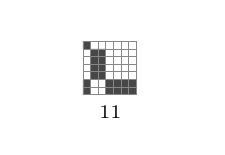
\begin{tikzpicture}[x=1mm,y=1mm,baseline=0mm]
\path[use as bounding box] (0,-.7) rectangle (21.5,11.9);
\begin{scope}[shift={(7.0,3.4)},x=0.97mm,y=0.97mm]
\fill[black!72] (0,6) rectangle (1,7) (1,5) rectangle (2,6) (2,5) rectangle (3,6) (1,4) rectangle (2,5) (2,4) rectangle (3,5) (1,3) rectangle (2,4) (2,3) rectangle (3,4) (1,2) rectangle (2,3) (2,2) rectangle (3,3) (0,1) rectangle (1,2) (3,1) rectangle (4,2) (4,1) rectangle (5,2) (5,1) rectangle (6,2) (6,1) rectangle (7,2) (0,0) rectangle (1,1) (3,0) rectangle (4,1) (4,0) rectangle (5,1) (5,0) rectangle (6,1) (6,0) rectangle (7,1);
\draw[black!47,line width=.16pt] (0,0)--(0,7) (0,0)--(7,0) (1,0)--(1,7) (0,1)--(7,1) (2,0)--(2,7) (0,2)--(7,2) (3,0)--(3,7) (0,3)--(7,3) (4,0)--(4,7) (0,4)--(7,4) (5,0)--(5,7) (0,5)--(7,5) (6,0)--(6,7) (0,6)--(7,6) (7,0)--(7,7) (0,7)--(7,7);
\end{scope}
\node[inner sep=0pt,font=\scriptsize] at (10.5,1.1) {$11$};
\end{tikzpicture} \\[.4mm]
\end{tabular}
\caption{Cross adjacencies tested in the connected case, part 1 of 2.}
\label{fig:nine-qfourteen-connected}
\end{figure}

\begin{figure}[!htbp]
\centering
\begin{tabular}{@{}c@{\hspace{1.6mm}}c@{\hspace{1.6mm}}c@{\hspace{1.6mm}}c@{\hspace{1.6mm}}c@{}}
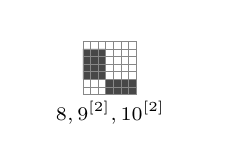
\begin{tikzpicture}[x=1mm,y=1mm,baseline=0mm]
\path[use as bounding box] (0,-.7) rectangle (21.5,11.9);
\begin{scope}[shift={(7.0,3.4)},x=0.97mm,y=0.97mm]
\fill[black!72] (0,5) rectangle (1,6) (1,5) rectangle (2,6) (2,5) rectangle (3,6) (0,4) rectangle (1,5) (1,4) rectangle (2,5) (2,4) rectangle (3,5) (0,3) rectangle (1,4) (1,3) rectangle (2,4) (2,3) rectangle (3,4) (0,2) rectangle (1,3) (1,2) rectangle (2,3) (2,2) rectangle (3,3) (3,1) rectangle (4,2) (4,1) rectangle (5,2) (5,1) rectangle (6,2) (6,1) rectangle (7,2) (3,0) rectangle (4,1) (4,0) rectangle (5,1) (5,0) rectangle (6,1) (6,0) rectangle (7,1);
\draw[black!47,line width=.16pt] (0,0)--(0,7) (0,0)--(7,0) (1,0)--(1,7) (0,1)--(7,1) (2,0)--(2,7) (0,2)--(7,2) (3,0)--(3,7) (0,3)--(7,3) (4,0)--(4,7) (0,4)--(7,4) (5,0)--(5,7) (0,5)--(7,5) (6,0)--(6,7) (0,6)--(7,6) (7,0)--(7,7) (0,7)--(7,7);
\end{scope}
\node[inner sep=0pt,font=\scriptsize] at (10.5,1.1) {$8,9^{[2]},10^{[2]}$};
\end{tikzpicture} &
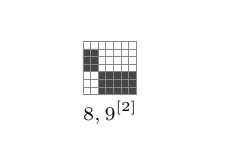
\begin{tikzpicture}[x=1mm,y=1mm,baseline=0mm]
\path[use as bounding box] (0,-.7) rectangle (21.5,11.9);
\begin{scope}[shift={(7.0,3.4)},x=0.97mm,y=0.97mm]
\fill[black!72] (0,5) rectangle (1,6) (1,5) rectangle (2,6) (0,4) rectangle (1,5) (1,4) rectangle (2,5) (0,3) rectangle (1,4) (1,3) rectangle (2,4) (2,2) rectangle (3,3) (3,2) rectangle (4,3) (4,2) rectangle (5,3) (5,2) rectangle (6,3) (6,2) rectangle (7,3) (2,1) rectangle (3,2) (3,1) rectangle (4,2) (4,1) rectangle (5,2) (5,1) rectangle (6,2) (6,1) rectangle (7,2) (2,0) rectangle (3,1) (3,0) rectangle (4,1) (4,0) rectangle (5,1) (5,0) rectangle (6,1) (6,0) rectangle (7,1);
\draw[black!47,line width=.16pt] (0,0)--(0,7) (0,0)--(7,0) (1,0)--(1,7) (0,1)--(7,1) (2,0)--(2,7) (0,2)--(7,2) (3,0)--(3,7) (0,3)--(7,3) (4,0)--(4,7) (0,4)--(7,4) (5,0)--(5,7) (0,5)--(7,5) (6,0)--(6,7) (0,6)--(7,6) (7,0)--(7,7) (0,7)--(7,7);
\end{scope}
\node[inner sep=0pt,font=\scriptsize] at (10.5,1.1) {$8,9^{[2]}$};
\end{tikzpicture} &
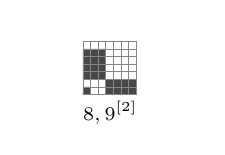
\begin{tikzpicture}[x=1mm,y=1mm,baseline=0mm]
\path[use as bounding box] (0,-.7) rectangle (21.5,11.9);
\begin{scope}[shift={(7.0,3.4)},x=0.97mm,y=0.97mm]
\fill[black!72] (0,5) rectangle (1,6) (1,5) rectangle (2,6) (2,5) rectangle (3,6) (0,4) rectangle (1,5) (1,4) rectangle (2,5) (2,4) rectangle (3,5) (0,3) rectangle (1,4) (1,3) rectangle (2,4) (2,3) rectangle (3,4) (0,2) rectangle (1,3) (1,2) rectangle (2,3) (2,2) rectangle (3,3) (3,1) rectangle (4,2) (4,1) rectangle (5,2) (5,1) rectangle (6,2) (6,1) rectangle (7,2) (0,0) rectangle (1,1) (3,0) rectangle (4,1) (4,0) rectangle (5,1) (5,0) rectangle (6,1) (6,0) rectangle (7,1);
\draw[black!47,line width=.16pt] (0,0)--(0,7) (0,0)--(7,0) (1,0)--(1,7) (0,1)--(7,1) (2,0)--(2,7) (0,2)--(7,2) (3,0)--(3,7) (0,3)--(7,3) (4,0)--(4,7) (0,4)--(7,4) (5,0)--(5,7) (0,5)--(7,5) (6,0)--(6,7) (0,6)--(7,6) (7,0)--(7,7) (0,7)--(7,7);
\end{scope}
\node[inner sep=0pt,font=\scriptsize] at (10.5,1.1) {$8,9^{[2]}$};
\end{tikzpicture} &
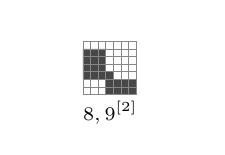
\begin{tikzpicture}[x=1mm,y=1mm,baseline=0mm]
\path[use as bounding box] (0,-.7) rectangle (21.5,11.9);
\begin{scope}[shift={(7.0,3.4)},x=0.97mm,y=0.97mm]
\fill[black!72] (0,5) rectangle (1,6) (1,5) rectangle (2,6) (2,5) rectangle (3,6) (0,4) rectangle (1,5) (1,4) rectangle (2,5) (2,4) rectangle (3,5) (0,3) rectangle (1,4) (1,3) rectangle (2,4) (2,3) rectangle (3,4) (0,2) rectangle (1,3) (1,2) rectangle (2,3) (2,2) rectangle (3,3) (3,2) rectangle (4,3) (3,1) rectangle (4,2) (4,1) rectangle (5,2) (5,1) rectangle (6,2) (6,1) rectangle (7,2) (3,0) rectangle (4,1) (4,0) rectangle (5,1) (5,0) rectangle (6,1) (6,0) rectangle (7,1);
\draw[black!47,line width=.16pt] (0,0)--(0,7) (0,0)--(7,0) (1,0)--(1,7) (0,1)--(7,1) (2,0)--(2,7) (0,2)--(7,2) (3,0)--(3,7) (0,3)--(7,3) (4,0)--(4,7) (0,4)--(7,4) (5,0)--(5,7) (0,5)--(7,5) (6,0)--(6,7) (0,6)--(7,6) (7,0)--(7,7) (0,7)--(7,7);
\end{scope}
\node[inner sep=0pt,font=\scriptsize] at (10.5,1.1) {$8,9^{[2]}$};
\end{tikzpicture} &
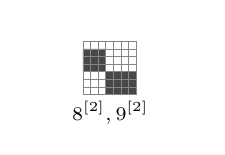
\begin{tikzpicture}[x=1mm,y=1mm,baseline=0mm]
\path[use as bounding box] (0,-.7) rectangle (21.5,11.9);
\begin{scope}[shift={(7.0,3.4)},x=0.97mm,y=0.97mm]
\fill[black!72] (0,5) rectangle (1,6) (1,5) rectangle (2,6) (2,5) rectangle (3,6) (0,4) rectangle (1,5) (1,4) rectangle (2,5) (2,4) rectangle (3,5) (0,3) rectangle (1,4) (1,3) rectangle (2,4) (2,3) rectangle (3,4) (3,2) rectangle (4,3) (4,2) rectangle (5,3) (5,2) rectangle (6,3) (6,2) rectangle (7,3) (3,1) rectangle (4,2) (4,1) rectangle (5,2) (5,1) rectangle (6,2) (6,1) rectangle (7,2) (3,0) rectangle (4,1) (4,0) rectangle (5,1) (5,0) rectangle (6,1) (6,0) rectangle (7,1);
\draw[black!47,line width=.16pt] (0,0)--(0,7) (0,0)--(7,0) (1,0)--(1,7) (0,1)--(7,1) (2,0)--(2,7) (0,2)--(7,2) (3,0)--(3,7) (0,3)--(7,3) (4,0)--(4,7) (0,4)--(7,4) (5,0)--(5,7) (0,5)--(7,5) (6,0)--(6,7) (0,6)--(7,6) (7,0)--(7,7) (0,7)--(7,7);
\end{scope}
\node[inner sep=0pt,font=\scriptsize] at (10.5,1.1) {$8^{[2]},9^{[2]}$};
\end{tikzpicture} \\[.4mm]
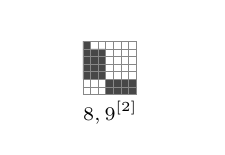
\begin{tikzpicture}[x=1mm,y=1mm,baseline=0mm]
\path[use as bounding box] (0,-.7) rectangle (21.5,11.9);
\begin{scope}[shift={(7.0,3.4)},x=0.97mm,y=0.97mm]
\fill[black!72] (0,6) rectangle (1,7) (0,5) rectangle (1,6) (1,5) rectangle (2,6) (2,5) rectangle (3,6) (0,4) rectangle (1,5) (1,4) rectangle (2,5) (2,4) rectangle (3,5) (0,3) rectangle (1,4) (1,3) rectangle (2,4) (2,3) rectangle (3,4) (0,2) rectangle (1,3) (1,2) rectangle (2,3) (2,2) rectangle (3,3) (3,1) rectangle (4,2) (4,1) rectangle (5,2) (5,1) rectangle (6,2) (6,1) rectangle (7,2) (3,0) rectangle (4,1) (4,0) rectangle (5,1) (5,0) rectangle (6,1) (6,0) rectangle (7,1);
\draw[black!47,line width=.16pt] (0,0)--(0,7) (0,0)--(7,0) (1,0)--(1,7) (0,1)--(7,1) (2,0)--(2,7) (0,2)--(7,2) (3,0)--(3,7) (0,3)--(7,3) (4,0)--(4,7) (0,4)--(7,4) (5,0)--(5,7) (0,5)--(7,5) (6,0)--(6,7) (0,6)--(7,6) (7,0)--(7,7) (0,7)--(7,7);
\end{scope}
\node[inner sep=0pt,font=\scriptsize] at (10.5,1.1) {$8,9^{[2]}$};
\end{tikzpicture} &
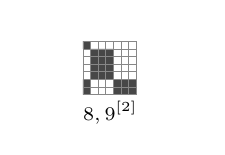
\begin{tikzpicture}[x=1mm,y=1mm,baseline=0mm]
\path[use as bounding box] (0,-.7) rectangle (21.5,11.9);
\begin{scope}[shift={(7.0,3.4)},x=0.97mm,y=0.97mm]
\fill[black!72] (0,6) rectangle (1,7) (1,5) rectangle (2,6) (2,5) rectangle (3,6) (3,5) rectangle (4,6) (1,4) rectangle (2,5) (2,4) rectangle (3,5) (3,4) rectangle (4,5) (1,3) rectangle (2,4) (2,3) rectangle (3,4) (3,3) rectangle (4,4) (1,2) rectangle (2,3) (2,2) rectangle (3,3) (3,2) rectangle (4,3) (0,1) rectangle (1,2) (4,1) rectangle (5,2) (5,1) rectangle (6,2) (6,1) rectangle (7,2) (0,0) rectangle (1,1) (4,0) rectangle (5,1) (5,0) rectangle (6,1) (6,0) rectangle (7,1);
\draw[black!47,line width=.16pt] (0,0)--(0,7) (0,0)--(7,0) (1,0)--(1,7) (0,1)--(7,1) (2,0)--(2,7) (0,2)--(7,2) (3,0)--(3,7) (0,3)--(7,3) (4,0)--(4,7) (0,4)--(7,4) (5,0)--(5,7) (0,5)--(7,5) (6,0)--(6,7) (0,6)--(7,6) (7,0)--(7,7) (0,7)--(7,7);
\end{scope}
\node[inner sep=0pt,font=\scriptsize] at (10.5,1.1) {$8,9^{[2]}$};
\end{tikzpicture} &
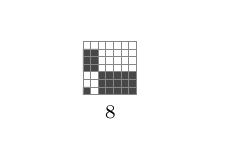
\begin{tikzpicture}[x=1mm,y=1mm,baseline=0mm]
\path[use as bounding box] (0,-.7) rectangle (21.5,11.9);
\begin{scope}[shift={(7.0,3.4)},x=0.97mm,y=0.97mm]
\fill[black!72] (0,5) rectangle (1,6) (1,5) rectangle (2,6) (0,4) rectangle (1,5) (1,4) rectangle (2,5) (0,3) rectangle (1,4) (1,3) rectangle (2,4) (2,2) rectangle (3,3) (3,2) rectangle (4,3) (4,2) rectangle (5,3) (5,2) rectangle (6,3) (6,2) rectangle (7,3) (2,1) rectangle (3,2) (3,1) rectangle (4,2) (4,1) rectangle (5,2) (5,1) rectangle (6,2) (6,1) rectangle (7,2) (0,0) rectangle (1,1) (2,0) rectangle (3,1) (3,0) rectangle (4,1) (4,0) rectangle (5,1) (5,0) rectangle (6,1) (6,0) rectangle (7,1);
\draw[black!47,line width=.16pt] (0,0)--(0,7) (0,0)--(7,0) (1,0)--(1,7) (0,1)--(7,1) (2,0)--(2,7) (0,2)--(7,2) (3,0)--(3,7) (0,3)--(7,3) (4,0)--(4,7) (0,4)--(7,4) (5,0)--(5,7) (0,5)--(7,5) (6,0)--(6,7) (0,6)--(7,6) (7,0)--(7,7) (0,7)--(7,7);
\end{scope}
\node[inner sep=0pt,font=\scriptsize] at (10.5,1.1) {$8$};
\end{tikzpicture} &
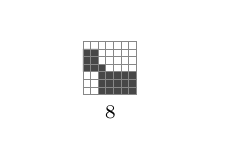
\begin{tikzpicture}[x=1mm,y=1mm,baseline=0mm]
\path[use as bounding box] (0,-.7) rectangle (21.5,11.9);
\begin{scope}[shift={(7.0,3.4)},x=0.97mm,y=0.97mm]
\fill[black!72] (0,5) rectangle (1,6) (1,5) rectangle (2,6) (0,4) rectangle (1,5) (1,4) rectangle (2,5) (0,3) rectangle (1,4) (1,3) rectangle (2,4) (2,3) rectangle (3,4) (2,2) rectangle (3,3) (3,2) rectangle (4,3) (4,2) rectangle (5,3) (5,2) rectangle (6,3) (6,2) rectangle (7,3) (2,1) rectangle (3,2) (3,1) rectangle (4,2) (4,1) rectangle (5,2) (5,1) rectangle (6,2) (6,1) rectangle (7,2) (2,0) rectangle (3,1) (3,0) rectangle (4,1) (4,0) rectangle (5,1) (5,0) rectangle (6,1) (6,0) rectangle (7,1);
\draw[black!47,line width=.16pt] (0,0)--(0,7) (0,0)--(7,0) (1,0)--(1,7) (0,1)--(7,1) (2,0)--(2,7) (0,2)--(7,2) (3,0)--(3,7) (0,3)--(7,3) (4,0)--(4,7) (0,4)--(7,4) (5,0)--(5,7) (0,5)--(7,5) (6,0)--(6,7) (0,6)--(7,6) (7,0)--(7,7) (0,7)--(7,7);
\end{scope}
\node[inner sep=0pt,font=\scriptsize] at (10.5,1.1) {$8$};
\end{tikzpicture} &
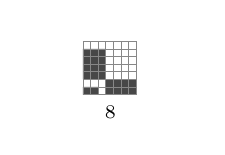
\begin{tikzpicture}[x=1mm,y=1mm,baseline=0mm]
\path[use as bounding box] (0,-.7) rectangle (21.5,11.9);
\begin{scope}[shift={(7.0,3.4)},x=0.97mm,y=0.97mm]
\fill[black!72] (0,5) rectangle (1,6) (1,5) rectangle (2,6) (2,5) rectangle (3,6) (0,4) rectangle (1,5) (1,4) rectangle (2,5) (2,4) rectangle (3,5) (0,3) rectangle (1,4) (1,3) rectangle (2,4) (2,3) rectangle (3,4) (0,2) rectangle (1,3) (1,2) rectangle (2,3) (2,2) rectangle (3,3) (3,1) rectangle (4,2) (4,1) rectangle (5,2) (5,1) rectangle (6,2) (6,1) rectangle (7,2) (0,0) rectangle (1,1) (1,0) rectangle (2,1) (3,0) rectangle (4,1) (4,0) rectangle (5,1) (5,0) rectangle (6,1) (6,0) rectangle (7,1);
\draw[black!47,line width=.16pt] (0,0)--(0,7) (0,0)--(7,0) (1,0)--(1,7) (0,1)--(7,1) (2,0)--(2,7) (0,2)--(7,2) (3,0)--(3,7) (0,3)--(7,3) (4,0)--(4,7) (0,4)--(7,4) (5,0)--(5,7) (0,5)--(7,5) (6,0)--(6,7) (0,6)--(7,6) (7,0)--(7,7) (0,7)--(7,7);
\end{scope}
\node[inner sep=0pt,font=\scriptsize] at (10.5,1.1) {$8$};
\end{tikzpicture} \\[.4mm]
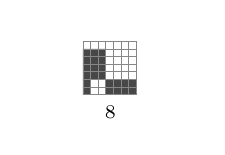
\begin{tikzpicture}[x=1mm,y=1mm,baseline=0mm]
\path[use as bounding box] (0,-.7) rectangle (21.5,11.9);
\begin{scope}[shift={(7.0,3.4)},x=0.97mm,y=0.97mm]
\fill[black!72] (0,5) rectangle (1,6) (1,5) rectangle (2,6) (2,5) rectangle (3,6) (0,4) rectangle (1,5) (1,4) rectangle (2,5) (2,4) rectangle (3,5) (0,3) rectangle (1,4) (1,3) rectangle (2,4) (2,3) rectangle (3,4) (0,2) rectangle (1,3) (1,2) rectangle (2,3) (2,2) rectangle (3,3) (0,1) rectangle (1,2) (3,1) rectangle (4,2) (4,1) rectangle (5,2) (5,1) rectangle (6,2) (6,1) rectangle (7,2) (0,0) rectangle (1,1) (3,0) rectangle (4,1) (4,0) rectangle (5,1) (5,0) rectangle (6,1) (6,0) rectangle (7,1);
\draw[black!47,line width=.16pt] (0,0)--(0,7) (0,0)--(7,0) (1,0)--(1,7) (0,1)--(7,1) (2,0)--(2,7) (0,2)--(7,2) (3,0)--(3,7) (0,3)--(7,3) (4,0)--(4,7) (0,4)--(7,4) (5,0)--(5,7) (0,5)--(7,5) (6,0)--(6,7) (0,6)--(7,6) (7,0)--(7,7) (0,7)--(7,7);
\end{scope}
\node[inner sep=0pt,font=\scriptsize] at (10.5,1.1) {$8$};
\end{tikzpicture} &
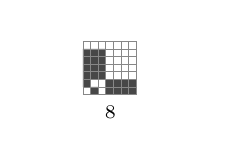
\begin{tikzpicture}[x=1mm,y=1mm,baseline=0mm]
\path[use as bounding box] (0,-.7) rectangle (21.5,11.9);
\begin{scope}[shift={(7.0,3.4)},x=0.97mm,y=0.97mm]
\fill[black!72] (0,5) rectangle (1,6) (1,5) rectangle (2,6) (2,5) rectangle (3,6) (0,4) rectangle (1,5) (1,4) rectangle (2,5) (2,4) rectangle (3,5) (0,3) rectangle (1,4) (1,3) rectangle (2,4) (2,3) rectangle (3,4) (0,2) rectangle (1,3) (1,2) rectangle (2,3) (2,2) rectangle (3,3) (0,1) rectangle (1,2) (3,1) rectangle (4,2) (4,1) rectangle (5,2) (5,1) rectangle (6,2) (6,1) rectangle (7,2) (1,0) rectangle (2,1) (3,0) rectangle (4,1) (4,0) rectangle (5,1) (5,0) rectangle (6,1) (6,0) rectangle (7,1);
\draw[black!47,line width=.16pt] (0,0)--(0,7) (0,0)--(7,0) (1,0)--(1,7) (0,1)--(7,1) (2,0)--(2,7) (0,2)--(7,2) (3,0)--(3,7) (0,3)--(7,3) (4,0)--(4,7) (0,4)--(7,4) (5,0)--(5,7) (0,5)--(7,5) (6,0)--(6,7) (0,6)--(7,6) (7,0)--(7,7) (0,7)--(7,7);
\end{scope}
\node[inner sep=0pt,font=\scriptsize] at (10.5,1.1) {$8$};
\end{tikzpicture} &
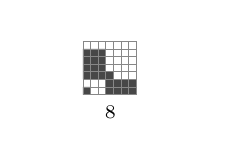
\begin{tikzpicture}[x=1mm,y=1mm,baseline=0mm]
\path[use as bounding box] (0,-.7) rectangle (21.5,11.9);
\begin{scope}[shift={(7.0,3.4)},x=0.97mm,y=0.97mm]
\fill[black!72] (0,5) rectangle (1,6) (1,5) rectangle (2,6) (2,5) rectangle (3,6) (0,4) rectangle (1,5) (1,4) rectangle (2,5) (2,4) rectangle (3,5) (0,3) rectangle (1,4) (1,3) rectangle (2,4) (2,3) rectangle (3,4) (0,2) rectangle (1,3) (1,2) rectangle (2,3) (2,2) rectangle (3,3) (3,2) rectangle (4,3) (3,1) rectangle (4,2) (4,1) rectangle (5,2) (5,1) rectangle (6,2) (6,1) rectangle (7,2) (0,0) rectangle (1,1) (3,0) rectangle (4,1) (4,0) rectangle (5,1) (5,0) rectangle (6,1) (6,0) rectangle (7,1);
\draw[black!47,line width=.16pt] (0,0)--(0,7) (0,0)--(7,0) (1,0)--(1,7) (0,1)--(7,1) (2,0)--(2,7) (0,2)--(7,2) (3,0)--(3,7) (0,3)--(7,3) (4,0)--(4,7) (0,4)--(7,4) (5,0)--(5,7) (0,5)--(7,5) (6,0)--(6,7) (0,6)--(7,6) (7,0)--(7,7) (0,7)--(7,7);
\end{scope}
\node[inner sep=0pt,font=\scriptsize] at (10.5,1.1) {$8$};
\end{tikzpicture} &
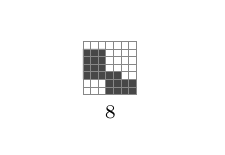
\begin{tikzpicture}[x=1mm,y=1mm,baseline=0mm]
\path[use as bounding box] (0,-.7) rectangle (21.5,11.9);
\begin{scope}[shift={(7.0,3.4)},x=0.97mm,y=0.97mm]
\fill[black!72] (0,5) rectangle (1,6) (1,5) rectangle (2,6) (2,5) rectangle (3,6) (0,4) rectangle (1,5) (1,4) rectangle (2,5) (2,4) rectangle (3,5) (0,3) rectangle (1,4) (1,3) rectangle (2,4) (2,3) rectangle (3,4) (0,2) rectangle (1,3) (1,2) rectangle (2,3) (2,2) rectangle (3,3) (3,2) rectangle (4,3) (4,2) rectangle (5,3) (3,1) rectangle (4,2) (4,1) rectangle (5,2) (5,1) rectangle (6,2) (6,1) rectangle (7,2) (3,0) rectangle (4,1) (4,0) rectangle (5,1) (5,0) rectangle (6,1) (6,0) rectangle (7,1);
\draw[black!47,line width=.16pt] (0,0)--(0,7) (0,0)--(7,0) (1,0)--(1,7) (0,1)--(7,1) (2,0)--(2,7) (0,2)--(7,2) (3,0)--(3,7) (0,3)--(7,3) (4,0)--(4,7) (0,4)--(7,4) (5,0)--(5,7) (0,5)--(7,5) (6,0)--(6,7) (0,6)--(7,6) (7,0)--(7,7) (0,7)--(7,7);
\end{scope}
\node[inner sep=0pt,font=\scriptsize] at (10.5,1.1) {$8$};
\end{tikzpicture} &
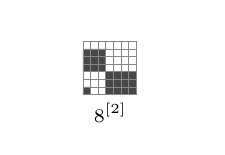
\begin{tikzpicture}[x=1mm,y=1mm,baseline=0mm]
\path[use as bounding box] (0,-.7) rectangle (21.5,11.9);
\begin{scope}[shift={(7.0,3.4)},x=0.97mm,y=0.97mm]
\fill[black!72] (0,5) rectangle (1,6) (1,5) rectangle (2,6) (2,5) rectangle (3,6) (0,4) rectangle (1,5) (1,4) rectangle (2,5) (2,4) rectangle (3,5) (0,3) rectangle (1,4) (1,3) rectangle (2,4) (2,3) rectangle (3,4) (3,2) rectangle (4,3) (4,2) rectangle (5,3) (5,2) rectangle (6,3) (6,2) rectangle (7,3) (3,1) rectangle (4,2) (4,1) rectangle (5,2) (5,1) rectangle (6,2) (6,1) rectangle (7,2) (0,0) rectangle (1,1) (3,0) rectangle (4,1) (4,0) rectangle (5,1) (5,0) rectangle (6,1) (6,0) rectangle (7,1);
\draw[black!47,line width=.16pt] (0,0)--(0,7) (0,0)--(7,0) (1,0)--(1,7) (0,1)--(7,1) (2,0)--(2,7) (0,2)--(7,2) (3,0)--(3,7) (0,3)--(7,3) (4,0)--(4,7) (0,4)--(7,4) (5,0)--(5,7) (0,5)--(7,5) (6,0)--(6,7) (0,6)--(7,6) (7,0)--(7,7) (0,7)--(7,7);
\end{scope}
\node[inner sep=0pt,font=\scriptsize] at (10.5,1.1) {$8^{[2]}$};
\end{tikzpicture} \\[.4mm]
\begin{tikzpicture}[x=1mm,y=1mm,baseline=0mm]
\path[use as bounding box] (0,-.7) rectangle (21.5,11.9);
\begin{scope}[shift={(7.0,3.4)},x=0.97mm,y=0.97mm]
\fill[black!72] (0,5) rectangle (1,6) (1,5) rectangle (2,6) (2,5) rectangle (3,6) (0,4) rectangle (1,5) (1,4) rectangle (2,5) (2,4) rectangle (3,5) (0,3) rectangle (1,4) (1,3) rectangle (2,4) (2,3) rectangle (3,4) (3,3) rectangle (4,4) (0,2) rectangle (1,3) (1,2) rectangle (2,3) (2,2) rectangle (3,3) (3,2) rectangle (4,3) (3,1) rectangle (4,2) (4,1) rectangle (5,2) (5,1) rectangle (6,2) (6,1) rectangle (7,2) (3,0) rectangle (4,1) (4,0) rectangle (5,1) (5,0) rectangle (6,1) (6,0) rectangle (7,1);
\draw[black!47,line width=.16pt] (0,0)--(0,7) (0,0)--(7,0) (1,0)--(1,7) (0,1)--(7,1) (2,0)--(2,7) (0,2)--(7,2) (3,0)--(3,7) (0,3)--(7,3) (4,0)--(4,7) (0,4)--(7,4) (5,0)--(5,7) (0,5)--(7,5) (6,0)--(6,7) (0,6)--(7,6) (7,0)--(7,7) (0,7)--(7,7);
\end{scope}
\node[inner sep=0pt,font=\scriptsize] at (10.5,1.1) {$8$};
\end{tikzpicture} &
\begin{tikzpicture}[x=1mm,y=1mm,baseline=0mm]
\path[use as bounding box] (0,-.7) rectangle (21.5,11.9);
\begin{scope}[shift={(7.0,3.4)},x=0.97mm,y=0.97mm]
\fill[black!72] (0,5) rectangle (1,6) (1,5) rectangle (2,6) (2,5) rectangle (3,6) (0,4) rectangle (1,5) (1,4) rectangle (2,5) (2,4) rectangle (3,5) (0,3) rectangle (1,4) (1,3) rectangle (2,4) (2,3) rectangle (3,4) (3,3) rectangle (4,4) (0,2) rectangle (1,3) (1,2) rectangle (2,3) (2,2) rectangle (3,3) (4,2) rectangle (5,3) (3,1) rectangle (4,2) (4,1) rectangle (5,2) (5,1) rectangle (6,2) (6,1) rectangle (7,2) (3,0) rectangle (4,1) (4,0) rectangle (5,1) (5,0) rectangle (6,1) (6,0) rectangle (7,1);
\draw[black!47,line width=.16pt] (0,0)--(0,7) (0,0)--(7,0) (1,0)--(1,7) (0,1)--(7,1) (2,0)--(2,7) (0,2)--(7,2) (3,0)--(3,7) (0,3)--(7,3) (4,0)--(4,7) (0,4)--(7,4) (5,0)--(5,7) (0,5)--(7,5) (6,0)--(6,7) (0,6)--(7,6) (7,0)--(7,7) (0,7)--(7,7);
\end{scope}
\node[inner sep=0pt,font=\scriptsize] at (10.5,1.1) {$8$};
\end{tikzpicture} &
\begin{tikzpicture}[x=1mm,y=1mm,baseline=0mm]
\path[use as bounding box] (0,-.7) rectangle (21.5,11.9);
\begin{scope}[shift={(7.0,3.4)},x=0.97mm,y=0.97mm]
\fill[black!72] (0,5) rectangle (1,6) (1,5) rectangle (2,6) (2,5) rectangle (3,6) (0,4) rectangle (1,5) (1,4) rectangle (2,5) (2,4) rectangle (3,5) (0,3) rectangle (1,4) (1,3) rectangle (2,4) (2,3) rectangle (3,4) (3,3) rectangle (4,4) (3,2) rectangle (4,3) (4,2) rectangle (5,3) (5,2) rectangle (6,3) (6,2) rectangle (7,3) (3,1) rectangle (4,2) (4,1) rectangle (5,2) (5,1) rectangle (6,2) (6,1) rectangle (7,2) (3,0) rectangle (4,1) (4,0) rectangle (5,1) (5,0) rectangle (6,1) (6,0) rectangle (7,1);
\draw[black!47,line width=.16pt] (0,0)--(0,7) (0,0)--(7,0) (1,0)--(1,7) (0,1)--(7,1) (2,0)--(2,7) (0,2)--(7,2) (3,0)--(3,7) (0,3)--(7,3) (4,0)--(4,7) (0,4)--(7,4) (5,0)--(5,7) (0,5)--(7,5) (6,0)--(6,7) (0,6)--(7,6) (7,0)--(7,7) (0,7)--(7,7);
\end{scope}
\node[inner sep=0pt,font=\scriptsize] at (10.5,1.1) {$8^{[2]}$};
\end{tikzpicture} &
\begin{tikzpicture}[x=1mm,y=1mm,baseline=0mm]
\path[use as bounding box] (0,-.7) rectangle (21.5,11.9);
\begin{scope}[shift={(7.0,3.4)},x=0.97mm,y=0.97mm]
\fill[black!72] (0,5) rectangle (1,6) (1,5) rectangle (2,6) (2,5) rectangle (3,6) (0,4) rectangle (1,5) (1,4) rectangle (2,5) (2,4) rectangle (3,5) (3,3) rectangle (4,4) (4,3) rectangle (5,4) (5,3) rectangle (6,4) (6,3) rectangle (7,4) (3,2) rectangle (4,3) (4,2) rectangle (5,3) (5,2) rectangle (6,3) (6,2) rectangle (7,3) (3,1) rectangle (4,2) (4,1) rectangle (5,2) (5,1) rectangle (6,2) (6,1) rectangle (7,2) (3,0) rectangle (4,1) (4,0) rectangle (5,1) (5,0) rectangle (6,1) (6,0) rectangle (7,1);
\draw[black!47,line width=.16pt] (0,0)--(0,7) (0,0)--(7,0) (1,0)--(1,7) (0,1)--(7,1) (2,0)--(2,7) (0,2)--(7,2) (3,0)--(3,7) (0,3)--(7,3) (4,0)--(4,7) (0,4)--(7,4) (5,0)--(5,7) (0,5)--(7,5) (6,0)--(6,7) (0,6)--(7,6) (7,0)--(7,7) (0,7)--(7,7);
\end{scope}
\node[inner sep=0pt,font=\scriptsize] at (10.5,1.1) {$8^{[2]}$};
\end{tikzpicture} &
\begin{tikzpicture}[x=1mm,y=1mm,baseline=0mm]
\path[use as bounding box] (0,-.7) rectangle (21.5,11.9);
\begin{scope}[shift={(7.0,3.4)},x=0.97mm,y=0.97mm]
\fill[black!72] (0,6) rectangle (1,7) (0,5) rectangle (1,6) (1,5) rectangle (2,6) (0,4) rectangle (1,5) (1,4) rectangle (2,5) (0,3) rectangle (1,4) (1,3) rectangle (2,4) (2,2) rectangle (3,3) (3,2) rectangle (4,3) (4,2) rectangle (5,3) (5,2) rectangle (6,3) (6,2) rectangle (7,3) (2,1) rectangle (3,2) (3,1) rectangle (4,2) (4,1) rectangle (5,2) (5,1) rectangle (6,2) (6,1) rectangle (7,2) (2,0) rectangle (3,1) (3,0) rectangle (4,1) (4,0) rectangle (5,1) (5,0) rectangle (6,1) (6,0) rectangle (7,1);
\draw[black!47,line width=.16pt] (0,0)--(0,7) (0,0)--(7,0) (1,0)--(1,7) (0,1)--(7,1) (2,0)--(2,7) (0,2)--(7,2) (3,0)--(3,7) (0,3)--(7,3) (4,0)--(4,7) (0,4)--(7,4) (5,0)--(5,7) (0,5)--(7,5) (6,0)--(6,7) (0,6)--(7,6) (7,0)--(7,7) (0,7)--(7,7);
\end{scope}
\node[inner sep=0pt,font=\scriptsize] at (10.5,1.1) {$8$};
\end{tikzpicture} \\[.4mm]
\begin{tikzpicture}[x=1mm,y=1mm,baseline=0mm]
\path[use as bounding box] (0,-.7) rectangle (21.5,11.9);
\begin{scope}[shift={(7.0,3.4)},x=0.97mm,y=0.97mm]
\fill[black!72] (0,6) rectangle (1,7) (1,5) rectangle (2,6) (2,5) rectangle (3,6) (1,4) rectangle (2,5) (2,4) rectangle (3,5) (1,3) rectangle (2,4) (2,3) rectangle (3,4) (0,2) rectangle (1,3) (3,2) rectangle (4,3) (4,2) rectangle (5,3) (5,2) rectangle (6,3) (6,2) rectangle (7,3) (0,1) rectangle (1,2) (3,1) rectangle (4,2) (4,1) rectangle (5,2) (5,1) rectangle (6,2) (6,1) rectangle (7,2) (0,0) rectangle (1,1) (3,0) rectangle (4,1) (4,0) rectangle (5,1) (5,0) rectangle (6,1) (6,0) rectangle (7,1);
\draw[black!47,line width=.16pt] (0,0)--(0,7) (0,0)--(7,0) (1,0)--(1,7) (0,1)--(7,1) (2,0)--(2,7) (0,2)--(7,2) (3,0)--(3,7) (0,3)--(7,3) (4,0)--(4,7) (0,4)--(7,4) (5,0)--(5,7) (0,5)--(7,5) (6,0)--(6,7) (0,6)--(7,6) (7,0)--(7,7) (0,7)--(7,7);
\end{scope}
\node[inner sep=0pt,font=\scriptsize] at (10.5,1.1) {$8$};
\end{tikzpicture} &
\begin{tikzpicture}[x=1mm,y=1mm,baseline=0mm]
\path[use as bounding box] (0,-.7) rectangle (21.5,11.9);
\begin{scope}[shift={(7.0,3.4)},x=0.97mm,y=0.97mm]
\fill[black!72] (0,6) rectangle (1,7) (0,5) rectangle (1,6) (1,5) rectangle (2,6) (2,5) rectangle (3,6) (0,4) rectangle (1,5) (1,4) rectangle (2,5) (2,4) rectangle (3,5) (0,3) rectangle (1,4) (1,3) rectangle (2,4) (2,3) rectangle (3,4) (0,2) rectangle (1,3) (1,2) rectangle (2,3) (2,2) rectangle (3,3) (3,1) rectangle (4,2) (4,1) rectangle (5,2) (5,1) rectangle (6,2) (6,1) rectangle (7,2) (0,0) rectangle (1,1) (3,0) rectangle (4,1) (4,0) rectangle (5,1) (5,0) rectangle (6,1) (6,0) rectangle (7,1);
\draw[black!47,line width=.16pt] (0,0)--(0,7) (0,0)--(7,0) (1,0)--(1,7) (0,1)--(7,1) (2,0)--(2,7) (0,2)--(7,2) (3,0)--(3,7) (0,3)--(7,3) (4,0)--(4,7) (0,4)--(7,4) (5,0)--(5,7) (0,5)--(7,5) (6,0)--(6,7) (0,6)--(7,6) (7,0)--(7,7) (0,7)--(7,7);
\end{scope}
\node[inner sep=0pt,font=\scriptsize] at (10.5,1.1) {$8$};
\end{tikzpicture} &
\begin{tikzpicture}[x=1mm,y=1mm,baseline=0mm]
\path[use as bounding box] (0,-.7) rectangle (21.5,11.9);
\begin{scope}[shift={(7.0,3.4)},x=0.97mm,y=0.97mm]
\fill[black!72] (0,6) rectangle (1,7) (0,5) rectangle (1,6) (1,5) rectangle (2,6) (2,5) rectangle (3,6) (0,4) rectangle (1,5) (1,4) rectangle (2,5) (2,4) rectangle (3,5) (0,3) rectangle (1,4) (1,3) rectangle (2,4) (2,3) rectangle (3,4) (0,2) rectangle (1,3) (1,2) rectangle (2,3) (2,2) rectangle (3,3) (3,1) rectangle (4,2) (4,1) rectangle (5,2) (5,1) rectangle (6,2) (6,1) rectangle (7,2) (1,0) rectangle (2,1) (3,0) rectangle (4,1) (4,0) rectangle (5,1) (5,0) rectangle (6,1) (6,0) rectangle (7,1);
\draw[black!47,line width=.16pt] (0,0)--(0,7) (0,0)--(7,0) (1,0)--(1,7) (0,1)--(7,1) (2,0)--(2,7) (0,2)--(7,2) (3,0)--(3,7) (0,3)--(7,3) (4,0)--(4,7) (0,4)--(7,4) (5,0)--(5,7) (0,5)--(7,5) (6,0)--(6,7) (0,6)--(7,6) (7,0)--(7,7) (0,7)--(7,7);
\end{scope}
\node[inner sep=0pt,font=\scriptsize] at (10.5,1.1) {$8^{[2]}$};
\end{tikzpicture} &
\begin{tikzpicture}[x=1mm,y=1mm,baseline=0mm]
\path[use as bounding box] (0,-.7) rectangle (21.5,11.9);
\begin{scope}[shift={(7.0,3.4)},x=0.97mm,y=0.97mm]
\fill[black!72] (0,6) rectangle (1,7) (0,5) rectangle (1,6) (1,5) rectangle (2,6) (2,5) rectangle (3,6) (0,4) rectangle (1,5) (1,4) rectangle (2,5) (2,4) rectangle (3,5) (0,3) rectangle (1,4) (1,3) rectangle (2,4) (2,3) rectangle (3,4) (0,2) rectangle (1,3) (1,2) rectangle (2,3) (2,2) rectangle (3,3) (3,2) rectangle (4,3) (3,1) rectangle (4,2) (4,1) rectangle (5,2) (5,1) rectangle (6,2) (6,1) rectangle (7,2) (3,0) rectangle (4,1) (4,0) rectangle (5,1) (5,0) rectangle (6,1) (6,0) rectangle (7,1);
\draw[black!47,line width=.16pt] (0,0)--(0,7) (0,0)--(7,0) (1,0)--(1,7) (0,1)--(7,1) (2,0)--(2,7) (0,2)--(7,2) (3,0)--(3,7) (0,3)--(7,3) (4,0)--(4,7) (0,4)--(7,4) (5,0)--(5,7) (0,5)--(7,5) (6,0)--(6,7) (0,6)--(7,6) (7,0)--(7,7) (0,7)--(7,7);
\end{scope}
\node[inner sep=0pt,font=\scriptsize] at (10.5,1.1) {$8$};
\end{tikzpicture} &
\begin{tikzpicture}[x=1mm,y=1mm,baseline=0mm]
\path[use as bounding box] (0,-.7) rectangle (21.5,11.9);
\begin{scope}[shift={(7.0,3.4)},x=0.97mm,y=0.97mm]
\fill[black!72] (0,6) rectangle (1,7) (0,5) rectangle (1,6) (1,5) rectangle (2,6) (2,5) rectangle (3,6) (0,4) rectangle (1,5) (1,4) rectangle (2,5) (2,4) rectangle (3,5) (0,3) rectangle (1,4) (1,3) rectangle (2,4) (2,3) rectangle (3,4) (3,2) rectangle (4,3) (4,2) rectangle (5,3) (5,2) rectangle (6,3) (6,2) rectangle (7,3) (3,1) rectangle (4,2) (4,1) rectangle (5,2) (5,1) rectangle (6,2) (6,1) rectangle (7,2) (3,0) rectangle (4,1) (4,0) rectangle (5,1) (5,0) rectangle (6,1) (6,0) rectangle (7,1);
\draw[black!47,line width=.16pt] (0,0)--(0,7) (0,0)--(7,0) (1,0)--(1,7) (0,1)--(7,1) (2,0)--(2,7) (0,2)--(7,2) (3,0)--(3,7) (0,3)--(7,3) (4,0)--(4,7) (0,4)--(7,4) (5,0)--(5,7) (0,5)--(7,5) (6,0)--(6,7) (0,6)--(7,6) (7,0)--(7,7) (0,7)--(7,7);
\end{scope}
\node[inner sep=0pt,font=\scriptsize] at (10.5,1.1) {$8^{[2]}$};
\end{tikzpicture} \\[.4mm]
\begin{tikzpicture}[x=1mm,y=1mm,baseline=0mm]
\path[use as bounding box] (0,-.7) rectangle (21.5,11.9);
\begin{scope}[shift={(7.0,3.4)},x=0.97mm,y=0.97mm]
\fill[black!72] (0,6) rectangle (1,7) (1,5) rectangle (2,6) (2,5) rectangle (3,6) (3,5) rectangle (4,6) (1,4) rectangle (2,5) (2,4) rectangle (3,5) (3,4) rectangle (4,5) (1,3) rectangle (2,4) (2,3) rectangle (3,4) (3,3) rectangle (4,4) (1,2) rectangle (2,3) (2,2) rectangle (3,3) (3,2) rectangle (4,3) (0,1) rectangle (1,2) (4,1) rectangle (5,2) (5,1) rectangle (6,2) (6,1) rectangle (7,2) (0,0) rectangle (1,1) (1,0) rectangle (2,1) (4,0) rectangle (5,1) (5,0) rectangle (6,1) (6,0) rectangle (7,1);
\draw[black!47,line width=.16pt] (0,0)--(0,7) (0,0)--(7,0) (1,0)--(1,7) (0,1)--(7,1) (2,0)--(2,7) (0,2)--(7,2) (3,0)--(3,7) (0,3)--(7,3) (4,0)--(4,7) (0,4)--(7,4) (5,0)--(5,7) (0,5)--(7,5) (6,0)--(6,7) (0,6)--(7,6) (7,0)--(7,7) (0,7)--(7,7);
\end{scope}
\node[inner sep=0pt,font=\scriptsize] at (10.5,1.1) {$8$};
\end{tikzpicture} &
\begin{tikzpicture}[x=1mm,y=1mm,baseline=0mm]
\path[use as bounding box] (0,-.7) rectangle (21.5,11.9);
\begin{scope}[shift={(7.0,3.4)},x=0.97mm,y=0.97mm]
\fill[black!72] (0,6) rectangle (1,7) (1,5) rectangle (2,6) (2,5) rectangle (3,6) (3,5) rectangle (4,6) (1,4) rectangle (2,5) (2,4) rectangle (3,5) (3,4) rectangle (4,5) (1,3) rectangle (2,4) (2,3) rectangle (3,4) (3,3) rectangle (4,4) (0,2) rectangle (1,3) (1,2) rectangle (2,3) (2,2) rectangle (3,3) (3,2) rectangle (4,3) (0,1) rectangle (1,2) (4,1) rectangle (5,2) (5,1) rectangle (6,2) (6,1) rectangle (7,2) (0,0) rectangle (1,1) (4,0) rectangle (5,1) (5,0) rectangle (6,1) (6,0) rectangle (7,1);
\draw[black!47,line width=.16pt] (0,0)--(0,7) (0,0)--(7,0) (1,0)--(1,7) (0,1)--(7,1) (2,0)--(2,7) (0,2)--(7,2) (3,0)--(3,7) (0,3)--(7,3) (4,0)--(4,7) (0,4)--(7,4) (5,0)--(5,7) (0,5)--(7,5) (6,0)--(6,7) (0,6)--(7,6) (7,0)--(7,7) (0,7)--(7,7);
\end{scope}
\node[inner sep=0pt,font=\scriptsize] at (10.5,1.1) {$8$};
\end{tikzpicture} &
\begin{tikzpicture}[x=1mm,y=1mm,baseline=0mm]
\path[use as bounding box] (0,-.7) rectangle (21.5,11.9);
\begin{scope}[shift={(7.0,3.4)},x=0.97mm,y=0.97mm]
\fill[black!72] (0,6) rectangle (1,7) (1,5) rectangle (2,6) (2,5) rectangle (3,6) (3,5) rectangle (4,6) (1,4) rectangle (2,5) (2,4) rectangle (3,5) (3,4) rectangle (4,5) (1,3) rectangle (2,4) (2,3) rectangle (3,4) (3,3) rectangle (4,4) (1,2) rectangle (2,3) (2,2) rectangle (3,3) (3,2) rectangle (4,3) (4,2) rectangle (5,3) (0,1) rectangle (1,2) (4,1) rectangle (5,2) (5,1) rectangle (6,2) (6,1) rectangle (7,2) (0,0) rectangle (1,1) (4,0) rectangle (5,1) (5,0) rectangle (6,1) (6,0) rectangle (7,1);
\draw[black!47,line width=.16pt] (0,0)--(0,7) (0,0)--(7,0) (1,0)--(1,7) (0,1)--(7,1) (2,0)--(2,7) (0,2)--(7,2) (3,0)--(3,7) (0,3)--(7,3) (4,0)--(4,7) (0,4)--(7,4) (5,0)--(5,7) (0,5)--(7,5) (6,0)--(6,7) (0,6)--(7,6) (7,0)--(7,7) (0,7)--(7,7);
\end{scope}
\node[inner sep=0pt,font=\scriptsize] at (10.5,1.1) {$8^{[2]}$};
\end{tikzpicture} &
\begin{tikzpicture}[x=1mm,y=1mm,baseline=0mm]
\path[use as bounding box] (0,-.7) rectangle (21.5,11.9);
\begin{scope}[shift={(7.0,3.4)},x=0.97mm,y=0.97mm]
\fill[black!72] (0,6) rectangle (1,7) (1,5) rectangle (2,6) (2,5) rectangle (3,6) (3,5) rectangle (4,6) (1,4) rectangle (2,5) (2,4) rectangle (3,5) (3,4) rectangle (4,5) (1,3) rectangle (2,4) (2,3) rectangle (3,4) (3,3) rectangle (4,4) (0,2) rectangle (1,3) (4,2) rectangle (5,3) (5,2) rectangle (6,3) (6,2) rectangle (7,3) (0,1) rectangle (1,2) (4,1) rectangle (5,2) (5,1) rectangle (6,2) (6,1) rectangle (7,2) (0,0) rectangle (1,1) (4,0) rectangle (5,1) (5,0) rectangle (6,1) (6,0) rectangle (7,1);
\draw[black!47,line width=.16pt] (0,0)--(0,7) (0,0)--(7,0) (1,0)--(1,7) (0,1)--(7,1) (2,0)--(2,7) (0,2)--(7,2) (3,0)--(3,7) (0,3)--(7,3) (4,0)--(4,7) (0,4)--(7,4) (5,0)--(5,7) (0,5)--(7,5) (6,0)--(6,7) (0,6)--(7,6) (7,0)--(7,7) (0,7)--(7,7);
\end{scope}
\node[inner sep=0pt,font=\scriptsize] at (10.5,1.1) {$8^{[2]}$};
\end{tikzpicture} &
\begin{tikzpicture}[x=1mm,y=1mm,baseline=0mm]
\path[use as bounding box] (0,-.7) rectangle (21.5,11.9);
\begin{scope}[shift={(7.0,3.4)},x=0.97mm,y=0.97mm]
\fill[black!72] (0,6) rectangle (1,7) (1,6) rectangle (2,7) (0,5) rectangle (1,6) (1,5) rectangle (2,6) (0,4) rectangle (1,5) (1,4) rectangle (2,5) (0,3) rectangle (1,4) (1,3) rectangle (2,4) (2,2) rectangle (3,3) (3,2) rectangle (4,3) (4,2) rectangle (5,3) (5,2) rectangle (6,3) (2,1) rectangle (3,2) (3,1) rectangle (4,2) (4,1) rectangle (5,2) (5,1) rectangle (6,2) (6,1) rectangle (7,2) (2,0) rectangle (3,1) (3,0) rectangle (4,1) (4,0) rectangle (5,1) (5,0) rectangle (6,1) (6,0) rectangle (7,1);
\draw[black!47,line width=.16pt] (0,0)--(0,7) (0,0)--(7,0) (1,0)--(1,7) (0,1)--(7,1) (2,0)--(2,7) (0,2)--(7,2) (3,0)--(3,7) (0,3)--(7,3) (4,0)--(4,7) (0,4)--(7,4) (5,0)--(5,7) (0,5)--(7,5) (6,0)--(6,7) (0,6)--(7,6) (7,0)--(7,7) (0,7)--(7,7);
\end{scope}
\node[inner sep=0pt,font=\scriptsize] at (10.5,1.1) {$8$};
\end{tikzpicture} \\[.4mm]
\begin{tikzpicture}[x=1mm,y=1mm,baseline=0mm]
\path[use as bounding box] (0,-.7) rectangle (21.5,11.9);
\begin{scope}[shift={(7.0,3.4)},x=0.97mm,y=0.97mm]
\fill[black!72] (0,6) rectangle (1,7) (1,6) rectangle (2,7) (0,5) rectangle (1,6) (1,5) rectangle (2,6) (0,4) rectangle (1,5) (1,4) rectangle (2,5) (0,3) rectangle (1,4) (1,3) rectangle (2,4) (2,3) rectangle (3,4) (3,2) rectangle (4,3) (4,2) rectangle (5,3) (5,2) rectangle (6,3) (6,2) rectangle (7,3) (3,1) rectangle (4,2) (4,1) rectangle (5,2) (5,1) rectangle (6,2) (6,1) rectangle (7,2) (2,0) rectangle (3,1) (3,0) rectangle (4,1) (4,0) rectangle (5,1) (5,0) rectangle (6,1) (6,0) rectangle (7,1);
\draw[black!47,line width=.16pt] (0,0)--(0,7) (0,0)--(7,0) (1,0)--(1,7) (0,1)--(7,1) (2,0)--(2,7) (0,2)--(7,2) (3,0)--(3,7) (0,3)--(7,3) (4,0)--(4,7) (0,4)--(7,4) (5,0)--(5,7) (0,5)--(7,5) (6,0)--(6,7) (0,6)--(7,6) (7,0)--(7,7) (0,7)--(7,7);
\end{scope}
\node[inner sep=0pt,font=\scriptsize] at (10.5,1.1) {$8$};
\end{tikzpicture} &
\begin{tikzpicture}[x=1mm,y=1mm,baseline=0mm]
\path[use as bounding box] (0,-.7) rectangle (21.5,11.9);
\begin{scope}[shift={(7.0,3.4)},x=0.97mm,y=0.97mm]
\fill[black!72] (0,6) rectangle (1,7) (1,6) rectangle (2,7) (0,5) rectangle (1,6) (1,5) rectangle (2,6) (0,4) rectangle (1,5) (1,4) rectangle (2,5) (2,4) rectangle (3,5) (0,3) rectangle (1,4) (1,3) rectangle (2,4) (2,3) rectangle (3,4) (3,2) rectangle (4,3) (4,2) rectangle (5,3) (5,2) rectangle (6,3) (6,2) rectangle (7,3) (3,1) rectangle (4,2) (4,1) rectangle (5,2) (5,1) rectangle (6,2) (6,1) rectangle (7,2) (3,0) rectangle (4,1) (4,0) rectangle (5,1) (5,0) rectangle (6,1) (6,0) rectangle (7,1);
\draw[black!47,line width=.16pt] (0,0)--(0,7) (0,0)--(7,0) (1,0)--(1,7) (0,1)--(7,1) (2,0)--(2,7) (0,2)--(7,2) (3,0)--(3,7) (0,3)--(7,3) (4,0)--(4,7) (0,4)--(7,4) (5,0)--(5,7) (0,5)--(7,5) (6,0)--(6,7) (0,6)--(7,6) (7,0)--(7,7) (0,7)--(7,7);
\end{scope}
\node[inner sep=0pt,font=\scriptsize] at (10.5,1.1) {$8$};
\end{tikzpicture} \\[.4mm]
\end{tabular}
\caption{Cross adjacencies tested in the connected case, part 2 of 2.}
\label{fig:nine-qfourteen-connected-last}
\end{figure}

\begin{figure}[!htbp]
\centering
\begin{tabular}{@{}c@{\hspace{1.6mm}}c@{\hspace{1.6mm}}c@{\hspace{1.6mm}}c@{\hspace{1.6mm}}c@{}}
\begin{tikzpicture}[x=1mm,y=1mm,baseline=0mm]
\path[use as bounding box] (0,-.7) rectangle (21.5,11.9);
\begin{scope}[shift={(7.0,3.4)},x=0.97mm,y=0.97mm]
\fill[black!72] (1,6) rectangle (2,7) (2,6) rectangle (3,7) (3,6) rectangle (4,7) (4,6) rectangle (5,7) (5,6) rectangle (6,7) (6,6) rectangle (7,7) (1,5) rectangle (2,6) (2,5) rectangle (3,6) (3,5) rectangle (4,6) (4,5) rectangle (5,6) (5,5) rectangle (6,6) (6,5) rectangle (7,6) (1,4) rectangle (2,5) (2,4) rectangle (3,5) (3,4) rectangle (4,5) (4,4) rectangle (5,5) (5,4) rectangle (6,5) (6,4) rectangle (7,5) (1,3) rectangle (2,4) (2,3) rectangle (3,4) (3,3) rectangle (4,4) (4,3) rectangle (5,4) (5,3) rectangle (6,4) (6,3) rectangle (7,4) (0,2) rectangle (1,3) (0,1) rectangle (1,2) (0,0) rectangle (1,1);
\draw[black!47,line width=.16pt] (0,0)--(0,7) (0,0)--(7,0) (1,0)--(1,7) (0,1)--(7,1) (2,0)--(2,7) (0,2)--(7,2) (3,0)--(3,7) (0,3)--(7,3) (4,0)--(4,7) (0,4)--(7,4) (5,0)--(5,7) (0,5)--(7,5) (6,0)--(6,7) (0,6)--(7,6) (7,0)--(7,7) (0,7)--(7,7);
\end{scope}
\node[inner sep=0pt,font=\scriptsize] at (10.5,1.1) {$0\!-\!3^{[2]}$};
\end{tikzpicture} &
\begin{tikzpicture}[x=1mm,y=1mm,baseline=0mm]
\path[use as bounding box] (0,-.7) rectangle (21.5,11.9);
\begin{scope}[shift={(7.0,3.4)},x=0.97mm,y=0.97mm]
\fill[black!72] (2,6) rectangle (3,7) (3,6) rectangle (4,7) (4,6) rectangle (5,7) (5,6) rectangle (6,7) (6,6) rectangle (7,7) (2,5) rectangle (3,6) (3,5) rectangle (4,6) (4,5) rectangle (5,6) (5,5) rectangle (6,6) (6,5) rectangle (7,6) (2,4) rectangle (3,5) (3,4) rectangle (4,5) (4,4) rectangle (5,5) (5,4) rectangle (6,5) (6,4) rectangle (7,5) (2,3) rectangle (3,4) (3,3) rectangle (4,4) (4,3) rectangle (5,4) (5,3) rectangle (6,4) (6,3) rectangle (7,4) (0,2) rectangle (1,3) (1,2) rectangle (2,3) (0,1) rectangle (1,2) (1,1) rectangle (2,2) (0,0) rectangle (1,1) (1,0) rectangle (2,1);
\draw[black!47,line width=.16pt] (0,0)--(0,7) (0,0)--(7,0) (1,0)--(1,7) (0,1)--(7,1) (2,0)--(2,7) (0,2)--(7,2) (3,0)--(3,7) (0,3)--(7,3) (4,0)--(4,7) (0,4)--(7,4) (5,0)--(5,7) (0,5)--(7,5) (6,0)--(6,7) (0,6)--(7,6) (7,0)--(7,7) (0,7)--(7,7);
\end{scope}
\node[inner sep=0pt,font=\scriptsize] at (10.5,1.1) {$0\!-\!4^{[2]}$};
\end{tikzpicture} &
\begin{tikzpicture}[x=1mm,y=1mm,baseline=0mm]
\path[use as bounding box] (0,-.7) rectangle (21.5,11.9);
\begin{scope}[shift={(7.0,3.4)},x=0.97mm,y=0.97mm]
\fill[black!72] (3,6) rectangle (4,7) (4,6) rectangle (5,7) (5,6) rectangle (6,7) (6,6) rectangle (7,7) (3,5) rectangle (4,6) (4,5) rectangle (5,6) (5,5) rectangle (6,6) (6,5) rectangle (7,6) (3,4) rectangle (4,5) (4,4) rectangle (5,5) (5,4) rectangle (6,5) (6,4) rectangle (7,5) (3,3) rectangle (4,4) (4,3) rectangle (5,4) (5,3) rectangle (6,4) (6,3) rectangle (7,4) (0,2) rectangle (1,3) (1,2) rectangle (2,3) (2,2) rectangle (3,3) (0,1) rectangle (1,2) (1,1) rectangle (2,2) (2,1) rectangle (3,2) (0,0) rectangle (1,1) (1,0) rectangle (2,1) (2,0) rectangle (3,1);
\draw[black!47,line width=.16pt] (0,0)--(0,7) (0,0)--(7,0) (1,0)--(1,7) (0,1)--(7,1) (2,0)--(2,7) (0,2)--(7,2) (3,0)--(3,7) (0,3)--(7,3) (4,0)--(4,7) (0,4)--(7,4) (5,0)--(5,7) (0,5)--(7,5) (6,0)--(6,7) (0,6)--(7,6) (7,0)--(7,7) (0,7)--(7,7);
\end{scope}
\node[inner sep=0pt,font=\scriptsize] at (10.5,1.1) {$0\!-\!5$};
\end{tikzpicture} &
\begin{tikzpicture}[x=1mm,y=1mm,baseline=0mm]
\path[use as bounding box] (0,-.7) rectangle (21.5,11.9);
\begin{scope}[shift={(7.0,3.4)},x=0.97mm,y=0.97mm]
\fill[black!72] (4,6) rectangle (5,7) (5,6) rectangle (6,7) (6,6) rectangle (7,7) (4,5) rectangle (5,6) (5,5) rectangle (6,6) (6,5) rectangle (7,6) (4,4) rectangle (5,5) (5,4) rectangle (6,5) (6,4) rectangle (7,5) (4,3) rectangle (5,4) (5,3) rectangle (6,4) (6,3) rectangle (7,4) (0,2) rectangle (1,3) (1,2) rectangle (2,3) (2,2) rectangle (3,3) (3,2) rectangle (4,3) (0,1) rectangle (1,2) (1,1) rectangle (2,2) (2,1) rectangle (3,2) (3,1) rectangle (4,2) (0,0) rectangle (1,1) (1,0) rectangle (2,1) (2,0) rectangle (3,1) (3,0) rectangle (4,1);
\draw[black!47,line width=.16pt] (0,0)--(0,7) (0,0)--(7,0) (1,0)--(1,7) (0,1)--(7,1) (2,0)--(2,7) (0,2)--(7,2) (3,0)--(3,7) (0,3)--(7,3) (4,0)--(4,7) (0,4)--(7,4) (5,0)--(5,7) (0,5)--(7,5) (6,0)--(6,7) (0,6)--(7,6) (7,0)--(7,7) (0,7)--(7,7);
\end{scope}
\node[inner sep=0pt,font=\scriptsize] at (10.5,1.1) {$0\!-\!6$};
\end{tikzpicture} &
\begin{tikzpicture}[x=1mm,y=1mm,baseline=0mm]
\path[use as bounding box] (0,-.7) rectangle (21.5,11.9);
\begin{scope}[shift={(7.0,3.4)},x=0.97mm,y=0.97mm]
\fill[black!72] (5,6) rectangle (6,7) (6,6) rectangle (7,7) (5,5) rectangle (6,6) (6,5) rectangle (7,6) (5,4) rectangle (6,5) (6,4) rectangle (7,5) (5,3) rectangle (6,4) (6,3) rectangle (7,4) (0,2) rectangle (1,3) (1,2) rectangle (2,3) (2,2) rectangle (3,3) (3,2) rectangle (4,3) (4,2) rectangle (5,3) (0,1) rectangle (1,2) (1,1) rectangle (2,2) (2,1) rectangle (3,2) (3,1) rectangle (4,2) (4,1) rectangle (5,2) (0,0) rectangle (1,1) (1,0) rectangle (2,1) (2,0) rectangle (3,1) (3,0) rectangle (4,1) (4,0) rectangle (5,1);
\draw[black!47,line width=.16pt] (0,0)--(0,7) (0,0)--(7,0) (1,0)--(1,7) (0,1)--(7,1) (2,0)--(2,7) (0,2)--(7,2) (3,0)--(3,7) (0,3)--(7,3) (4,0)--(4,7) (0,4)--(7,4) (5,0)--(5,7) (0,5)--(7,5) (6,0)--(6,7) (0,6)--(7,6) (7,0)--(7,7) (0,7)--(7,7);
\end{scope}
\node[inner sep=0pt,font=\scriptsize] at (10.5,1.1) {$0\!-\!7^{[2]}$};
\end{tikzpicture} \\[.4mm]
\begin{tikzpicture}[x=1mm,y=1mm,baseline=0mm]
\path[use as bounding box] (0,-.7) rectangle (21.5,11.9);
\begin{scope}[shift={(7.0,3.4)},x=0.97mm,y=0.97mm]
\fill[black!72] (2,6) rectangle (3,7) (3,6) rectangle (4,7) (4,6) rectangle (5,7) (5,6) rectangle (6,7) (6,6) rectangle (7,7) (2,5) rectangle (3,6) (3,5) rectangle (4,6) (4,5) rectangle (5,6) (5,5) rectangle (6,6) (6,5) rectangle (7,6) (2,4) rectangle (3,5) (3,4) rectangle (4,5) (4,4) rectangle (5,5) (5,4) rectangle (6,5) (6,4) rectangle (7,5) (2,3) rectangle (3,4) (3,3) rectangle (4,4) (4,3) rectangle (5,4) (5,3) rectangle (6,4) (6,3) rectangle (7,4) (2,2) rectangle (3,3) (3,2) rectangle (4,3) (4,2) rectangle (5,3) (5,2) rectangle (6,3) (6,2) rectangle (7,3) (0,1) rectangle (1,2) (1,1) rectangle (2,2) (0,0) rectangle (1,1) (1,0) rectangle (2,1);
\draw[black!47,line width=.16pt] (0,0)--(0,7) (0,0)--(7,0) (1,0)--(1,7) (0,1)--(7,1) (2,0)--(2,7) (0,2)--(7,2) (3,0)--(3,7) (0,3)--(7,3) (4,0)--(4,7) (0,4)--(7,4) (5,0)--(5,7) (0,5)--(7,5) (6,0)--(6,7) (0,6)--(7,6) (7,0)--(7,7) (0,7)--(7,7);
\end{scope}
\node[inner sep=0pt,font=\scriptsize] at (10.5,1.1) {$0\!-\!1$};
\end{tikzpicture} &
\begin{tikzpicture}[x=1mm,y=1mm,baseline=0mm]
\path[use as bounding box] (0,-.7) rectangle (21.5,11.9);
\begin{scope}[shift={(7.0,3.4)},x=0.97mm,y=0.97mm]
\fill[black!72] (3,6) rectangle (4,7) (4,6) rectangle (5,7) (5,6) rectangle (6,7) (6,6) rectangle (7,7) (3,5) rectangle (4,6) (4,5) rectangle (5,6) (5,5) rectangle (6,6) (6,5) rectangle (7,6) (3,4) rectangle (4,5) (4,4) rectangle (5,5) (5,4) rectangle (6,5) (6,4) rectangle (7,5) (0,3) rectangle (1,4) (1,3) rectangle (2,4) (2,3) rectangle (3,4) (6,3) rectangle (7,4) (0,2) rectangle (1,3) (1,2) rectangle (2,3) (2,2) rectangle (3,3) (6,2) rectangle (7,3) (0,1) rectangle (1,2) (1,1) rectangle (2,2) (2,1) rectangle (3,2) (6,1) rectangle (7,2) (0,0) rectangle (1,1) (1,0) rectangle (2,1) (2,0) rectangle (3,1) (3,0) rectangle (4,1) (4,0) rectangle (5,1) (5,0) rectangle (6,1);
\draw[black!47,line width=.16pt] (0,0)--(0,7) (0,0)--(7,0) (1,0)--(1,7) (0,1)--(7,1) (2,0)--(2,7) (0,2)--(7,2) (3,0)--(3,7) (0,3)--(7,3) (4,0)--(4,7) (0,4)--(7,4) (5,0)--(5,7) (0,5)--(7,5) (6,0)--(6,7) (0,6)--(7,6) (7,0)--(7,7) (0,7)--(7,7);
\end{scope}
\node[inner sep=0pt,font=\scriptsize] at (10.5,1.1) {$0$};
\end{tikzpicture} &
\begin{tikzpicture}[x=1mm,y=1mm,baseline=0mm]
\path[use as bounding box] (0,-.7) rectangle (21.5,11.9);
\begin{scope}[shift={(7.0,3.4)},x=0.97mm,y=0.97mm]
\fill[black!72] (4,6) rectangle (5,7) (5,6) rectangle (6,7) (6,6) rectangle (7,7) (4,5) rectangle (5,6) (5,5) rectangle (6,6) (6,5) rectangle (7,6) (4,4) rectangle (5,5) (5,4) rectangle (6,5) (6,4) rectangle (7,5) (0,3) rectangle (1,4) (1,3) rectangle (2,4) (2,3) rectangle (3,4) (3,3) rectangle (4,4) (6,3) rectangle (7,4) (0,2) rectangle (1,3) (1,2) rectangle (2,3) (2,2) rectangle (3,3) (3,2) rectangle (4,3) (6,2) rectangle (7,3) (0,1) rectangle (1,2) (1,1) rectangle (2,2) (2,1) rectangle (3,2) (3,1) rectangle (4,2) (6,1) rectangle (7,2) (0,0) rectangle (1,1) (1,0) rectangle (2,1) (2,0) rectangle (3,1) (3,0) rectangle (4,1) (4,0) rectangle (5,1) (5,0) rectangle (6,1);
\draw[black!47,line width=.16pt] (0,0)--(0,7) (0,0)--(7,0) (1,0)--(1,7) (0,1)--(7,1) (2,0)--(2,7) (0,2)--(7,2) (3,0)--(3,7) (0,3)--(7,3) (4,0)--(4,7) (0,4)--(7,4) (5,0)--(5,7) (0,5)--(7,5) (6,0)--(6,7) (0,6)--(7,6) (7,0)--(7,7) (0,7)--(7,7);
\end{scope}
\node[inner sep=0pt,font=\scriptsize] at (10.5,1.1) {$0^{[2]}$};
\end{tikzpicture} &
\begin{tikzpicture}[x=1mm,y=1mm,baseline=0mm]
\path[use as bounding box] (0,-.7) rectangle (21.5,11.9);
\begin{scope}[shift={(7.0,3.4)},x=0.97mm,y=0.97mm]
\fill[black!72] (4,6) rectangle (5,7) (5,6) rectangle (6,7) (6,6) rectangle (7,7) (4,5) rectangle (5,6) (5,5) rectangle (6,6) (6,5) rectangle (7,6) (4,4) rectangle (5,5) (5,4) rectangle (6,5) (6,4) rectangle (7,5) (0,3) rectangle (1,4) (1,3) rectangle (2,4) (2,3) rectangle (3,4) (3,3) rectangle (4,4) (0,2) rectangle (1,3) (1,2) rectangle (2,3) (2,2) rectangle (3,3) (3,2) rectangle (4,3) (0,1) rectangle (1,2) (1,1) rectangle (2,2) (2,1) rectangle (3,2) (3,1) rectangle (4,2) (0,0) rectangle (1,1) (1,0) rectangle (2,1) (2,0) rectangle (3,1) (3,0) rectangle (4,1) (4,0) rectangle (5,1) (5,0) rectangle (6,1) (6,0) rectangle (7,1);
\draw[black!47,line width=.16pt] (0,0)--(0,7) (0,0)--(7,0) (1,0)--(1,7) (0,1)--(7,1) (2,0)--(2,7) (0,2)--(7,2) (3,0)--(3,7) (0,3)--(7,3) (4,0)--(4,7) (0,4)--(7,4) (5,0)--(5,7) (0,5)--(7,5) (6,0)--(6,7) (0,6)--(7,6) (7,0)--(7,7) (0,7)--(7,7);
\end{scope}
\node[inner sep=0pt,font=\scriptsize] at (10.5,1.1) {$0\!-\!2^{[2]}$};
\end{tikzpicture} &
\begin{tikzpicture}[x=1mm,y=1mm,baseline=0mm]
\path[use as bounding box] (0,-.7) rectangle (21.5,11.9);
\begin{scope}[shift={(7.0,3.4)},x=0.97mm,y=0.97mm]
\fill[black!72] (5,6) rectangle (6,7) (6,6) rectangle (7,7) (5,5) rectangle (6,6) (6,5) rectangle (7,6) (5,4) rectangle (6,5) (6,4) rectangle (7,5) (0,3) rectangle (1,4) (1,3) rectangle (2,4) (2,3) rectangle (3,4) (3,3) rectangle (4,4) (4,3) rectangle (5,4) (6,3) rectangle (7,4) (0,2) rectangle (1,3) (1,2) rectangle (2,3) (2,2) rectangle (3,3) (3,2) rectangle (4,3) (4,2) rectangle (5,3) (6,2) rectangle (7,3) (0,1) rectangle (1,2) (1,1) rectangle (2,2) (2,1) rectangle (3,2) (3,1) rectangle (4,2) (4,1) rectangle (5,2) (5,1) rectangle (6,2) (0,0) rectangle (1,1) (1,0) rectangle (2,1) (2,0) rectangle (3,1) (3,0) rectangle (4,1) (4,0) rectangle (5,1) (5,0) rectangle (6,1);
\draw[black!47,line width=.16pt] (0,0)--(0,7) (0,0)--(7,0) (1,0)--(1,7) (0,1)--(7,1) (2,0)--(2,7) (0,2)--(7,2) (3,0)--(3,7) (0,3)--(7,3) (4,0)--(4,7) (0,4)--(7,4) (5,0)--(5,7) (0,5)--(7,5) (6,0)--(6,7) (0,6)--(7,6) (7,0)--(7,7) (0,7)--(7,7);
\end{scope}
\node[inner sep=0pt,font=\scriptsize] at (10.5,1.1) {$0^{[2]}$};
\end{tikzpicture} \\[.4mm]
\begin{tikzpicture}[x=1mm,y=1mm,baseline=0mm]
\path[use as bounding box] (0,-.7) rectangle (21.5,11.9);
\begin{scope}[shift={(7.0,3.4)},x=0.97mm,y=0.97mm]
\fill[black!72] (5,6) rectangle (6,7) (6,6) rectangle (7,7) (5,5) rectangle (6,6) (6,5) rectangle (7,6) (5,4) rectangle (6,5) (6,4) rectangle (7,5) (0,3) rectangle (1,4) (1,3) rectangle (2,4) (2,3) rectangle (3,4) (3,3) rectangle (4,4) (4,3) rectangle (5,4) (6,3) rectangle (7,4) (0,2) rectangle (1,3) (1,2) rectangle (2,3) (2,2) rectangle (3,3) (3,2) rectangle (4,3) (4,2) rectangle (5,3) (6,2) rectangle (7,3) (0,1) rectangle (1,2) (1,1) rectangle (2,2) (2,1) rectangle (3,2) (3,1) rectangle (4,2) (4,1) rectangle (5,2) (6,1) rectangle (7,2) (0,0) rectangle (1,1) (1,0) rectangle (2,1) (2,0) rectangle (3,1) (3,0) rectangle (4,1) (4,0) rectangle (5,1) (5,0) rectangle (6,1);
\draw[black!47,line width=.16pt] (0,0)--(0,7) (0,0)--(7,0) (1,0)--(1,7) (0,1)--(7,1) (2,0)--(2,7) (0,2)--(7,2) (3,0)--(3,7) (0,3)--(7,3) (4,0)--(4,7) (0,4)--(7,4) (5,0)--(5,7) (0,5)--(7,5) (6,0)--(6,7) (0,6)--(7,6) (7,0)--(7,7) (0,7)--(7,7);
\end{scope}
\node[inner sep=0pt,font=\scriptsize] at (10.5,1.1) {$0^{[2]}$};
\end{tikzpicture} &
\begin{tikzpicture}[x=1mm,y=1mm,baseline=0mm]
\path[use as bounding box] (0,-.7) rectangle (21.5,11.9);
\begin{scope}[shift={(7.0,3.4)},x=0.97mm,y=0.97mm]
\fill[black!72] (5,6) rectangle (6,7) (6,6) rectangle (7,7) (5,5) rectangle (6,6) (6,5) rectangle (7,6) (5,4) rectangle (6,5) (6,4) rectangle (7,5) (0,3) rectangle (1,4) (1,3) rectangle (2,4) (2,3) rectangle (3,4) (3,3) rectangle (4,4) (4,3) rectangle (5,4) (0,2) rectangle (1,3) (1,2) rectangle (2,3) (2,2) rectangle (3,3) (3,2) rectangle (4,3) (4,2) rectangle (5,3) (0,1) rectangle (1,2) (1,1) rectangle (2,2) (2,1) rectangle (3,2) (3,1) rectangle (4,2) (4,1) rectangle (5,2) (0,0) rectangle (1,1) (1,0) rectangle (2,1) (2,0) rectangle (3,1) (3,0) rectangle (4,1) (4,0) rectangle (5,1) (5,0) rectangle (6,1) (6,0) rectangle (7,1);
\draw[black!47,line width=.16pt] (0,0)--(0,7) (0,0)--(7,0) (1,0)--(1,7) (0,1)--(7,1) (2,0)--(2,7) (0,2)--(7,2) (3,0)--(3,7) (0,3)--(7,3) (4,0)--(4,7) (0,4)--(7,4) (5,0)--(5,7) (0,5)--(7,5) (6,0)--(6,7) (0,6)--(7,6) (7,0)--(7,7) (0,7)--(7,7);
\end{scope}
\node[inner sep=0pt,font=\scriptsize] at (10.5,1.1) {$0\!-\!2^{[2]}$};
\end{tikzpicture} &
\begin{tikzpicture}[x=1mm,y=1mm,baseline=0mm]
\path[use as bounding box] (0,-.7) rectangle (21.5,11.9);
\begin{scope}[shift={(7.0,3.4)},x=0.97mm,y=0.97mm]
\fill[black!72] (6,6) rectangle (7,7) (6,5) rectangle (7,6) (6,4) rectangle (7,5) (0,3) rectangle (1,4) (1,3) rectangle (2,4) (2,3) rectangle (3,4) (3,3) rectangle (4,4) (4,3) rectangle (5,4) (5,3) rectangle (6,4) (0,2) rectangle (1,3) (1,2) rectangle (2,3) (2,2) rectangle (3,3) (3,2) rectangle (4,3) (4,2) rectangle (5,3) (5,2) rectangle (6,3) (0,1) rectangle (1,2) (1,1) rectangle (2,2) (2,1) rectangle (3,2) (3,1) rectangle (4,2) (4,1) rectangle (5,2) (5,1) rectangle (6,2) (0,0) rectangle (1,1) (1,0) rectangle (2,1) (2,0) rectangle (3,1) (3,0) rectangle (4,1) (4,0) rectangle (5,1) (5,0) rectangle (6,1) (6,0) rectangle (7,1);
\draw[black!47,line width=.16pt] (0,0)--(0,7) (0,0)--(7,0) (1,0)--(1,7) (0,1)--(7,1) (2,0)--(2,7) (0,2)--(7,2) (3,0)--(3,7) (0,3)--(7,3) (4,0)--(4,7) (0,4)--(7,4) (5,0)--(5,7) (0,5)--(7,5) (6,0)--(6,7) (0,6)--(7,6) (7,0)--(7,7) (0,7)--(7,7);
\end{scope}
\node[inner sep=0pt,font=\scriptsize] at (10.5,1.1) {$0\!-\!2^{[2]}$};
\end{tikzpicture} &
\begin{tikzpicture}[x=1mm,y=1mm,baseline=0mm]
\path[use as bounding box] (0,-.7) rectangle (21.5,11.9);
\begin{scope}[shift={(7.0,3.4)},x=0.97mm,y=0.97mm]
\fill[black!72] (1,6) rectangle (2,7) (2,6) rectangle (3,7) (3,6) rectangle (4,7) (4,6) rectangle (5,7) (5,6) rectangle (6,7) (6,6) rectangle (7,7) (1,5) rectangle (2,6) (2,5) rectangle (3,6) (3,5) rectangle (4,6) (4,5) rectangle (5,6) (5,5) rectangle (6,6) (6,5) rectangle (7,6) (1,4) rectangle (2,5) (2,4) rectangle (3,5) (3,4) rectangle (4,5) (4,4) rectangle (5,5) (5,4) rectangle (6,5) (6,4) rectangle (7,5) (1,3) rectangle (2,4) (2,3) rectangle (3,4) (3,3) rectangle (4,4) (4,3) rectangle (5,4) (5,3) rectangle (6,4) (6,3) rectangle (7,4) (0,2) rectangle (1,3) (6,2) rectangle (7,3) (0,1) rectangle (1,2) (6,1) rectangle (7,2) (0,0) rectangle (1,1) (6,0) rectangle (7,1);
\draw[black!47,line width=.16pt] (0,0)--(0,7) (0,0)--(7,0) (1,0)--(1,7) (0,1)--(7,1) (2,0)--(2,7) (0,2)--(7,2) (3,0)--(3,7) (0,3)--(7,3) (4,0)--(4,7) (0,4)--(7,4) (5,0)--(5,7) (0,5)--(7,5) (6,0)--(6,7) (0,6)--(7,6) (7,0)--(7,7) (0,7)--(7,7);
\end{scope}
\node[inner sep=0pt,font=\scriptsize] at (10.5,1.1) {$0^{[2]}$};
\end{tikzpicture} &
\begin{tikzpicture}[x=1mm,y=1mm,baseline=0mm]
\path[use as bounding box] (0,-.7) rectangle (21.5,11.9);
\begin{scope}[shift={(7.0,3.4)},x=0.97mm,y=0.97mm]
\fill[black!72] (2,6) rectangle (3,7) (3,6) rectangle (4,7) (4,6) rectangle (5,7) (5,6) rectangle (6,7) (6,6) rectangle (7,7) (2,5) rectangle (3,6) (3,5) rectangle (4,6) (4,5) rectangle (5,6) (5,5) rectangle (6,6) (6,5) rectangle (7,6) (2,4) rectangle (3,5) (3,4) rectangle (4,5) (4,4) rectangle (5,5) (5,4) rectangle (6,5) (6,4) rectangle (7,5) (2,3) rectangle (3,4) (3,3) rectangle (4,4) (4,3) rectangle (5,4) (5,3) rectangle (6,4) (6,3) rectangle (7,4) (0,2) rectangle (1,3) (1,2) rectangle (2,3) (6,2) rectangle (7,3) (0,1) rectangle (1,2) (1,1) rectangle (2,2) (6,1) rectangle (7,2) (0,0) rectangle (1,1) (1,0) rectangle (2,1) (6,0) rectangle (7,1);
\draw[black!47,line width=.16pt] (0,0)--(0,7) (0,0)--(7,0) (1,0)--(1,7) (0,1)--(7,1) (2,0)--(2,7) (0,2)--(7,2) (3,0)--(3,7) (0,3)--(7,3) (4,0)--(4,7) (0,4)--(7,4) (5,0)--(5,7) (0,5)--(7,5) (6,0)--(6,7) (0,6)--(7,6) (7,0)--(7,7) (0,7)--(7,7);
\end{scope}
\node[inner sep=0pt,font=\scriptsize] at (10.5,1.1) {$0\!-\!1^{[2]}$};
\end{tikzpicture} \\[.4mm]
\begin{tikzpicture}[x=1mm,y=1mm,baseline=0mm]
\path[use as bounding box] (0,-.7) rectangle (21.5,11.9);
\begin{scope}[shift={(7.0,3.4)},x=0.97mm,y=0.97mm]
\fill[black!72] (4,6) rectangle (5,7) (5,6) rectangle (6,7) (6,6) rectangle (7,7) (4,5) rectangle (5,6) (5,5) rectangle (6,6) (6,5) rectangle (7,6) (4,4) rectangle (5,5) (5,4) rectangle (6,5) (6,4) rectangle (7,5) (4,3) rectangle (5,4) (5,3) rectangle (6,4) (6,3) rectangle (7,4) (0,2) rectangle (1,3) (1,2) rectangle (2,3) (2,2) rectangle (3,3) (3,2) rectangle (4,3) (5,2) rectangle (6,3) (6,2) rectangle (7,3) (0,1) rectangle (1,2) (1,1) rectangle (2,2) (2,1) rectangle (3,2) (3,1) rectangle (4,2) (5,1) rectangle (6,2) (6,1) rectangle (7,2) (0,0) rectangle (1,1) (1,0) rectangle (2,1) (2,0) rectangle (3,1) (3,0) rectangle (4,1) (4,0) rectangle (5,1);
\draw[black!47,line width=.16pt] (0,0)--(0,7) (0,0)--(7,0) (1,0)--(1,7) (0,1)--(7,1) (2,0)--(2,7) (0,2)--(7,2) (3,0)--(3,7) (0,3)--(7,3) (4,0)--(4,7) (0,4)--(7,4) (5,0)--(5,7) (0,5)--(7,5) (6,0)--(6,7) (0,6)--(7,6) (7,0)--(7,7) (0,7)--(7,7);
\end{scope}
\node[inner sep=0pt,font=\scriptsize] at (10.5,1.1) {$0\!-\!1$};
\end{tikzpicture} &
\begin{tikzpicture}[x=1mm,y=1mm,baseline=0mm]
\path[use as bounding box] (0,-.7) rectangle (21.5,11.9);
\begin{scope}[shift={(7.0,3.4)},x=0.97mm,y=0.97mm]
\fill[black!72] (4,6) rectangle (5,7) (5,6) rectangle (6,7) (6,6) rectangle (7,7) (4,5) rectangle (5,6) (5,5) rectangle (6,6) (6,5) rectangle (7,6) (4,4) rectangle (5,5) (5,4) rectangle (6,5) (6,4) rectangle (7,5) (4,3) rectangle (5,4) (5,3) rectangle (6,4) (6,3) rectangle (7,4) (0,2) rectangle (1,3) (1,2) rectangle (2,3) (2,2) rectangle (3,3) (3,2) rectangle (4,3) (6,2) rectangle (7,3) (0,1) rectangle (1,2) (1,1) rectangle (2,2) (2,1) rectangle (3,2) (3,1) rectangle (4,2) (6,1) rectangle (7,2) (0,0) rectangle (1,1) (1,0) rectangle (2,1) (2,0) rectangle (3,1) (3,0) rectangle (4,1) (4,0) rectangle (5,1) (5,0) rectangle (6,1);
\draw[black!47,line width=.16pt] (0,0)--(0,7) (0,0)--(7,0) (1,0)--(1,7) (0,1)--(7,1) (2,0)--(2,7) (0,2)--(7,2) (3,0)--(3,7) (0,3)--(7,3) (4,0)--(4,7) (0,4)--(7,4) (5,0)--(5,7) (0,5)--(7,5) (6,0)--(6,7) (0,6)--(7,6) (7,0)--(7,7) (0,7)--(7,7);
\end{scope}
\node[inner sep=0pt,font=\scriptsize] at (10.5,1.1) {$0\!-\!2$};
\end{tikzpicture} &
\begin{tikzpicture}[x=1mm,y=1mm,baseline=0mm]
\path[use as bounding box] (0,-.7) rectangle (21.5,11.9);
\begin{scope}[shift={(7.0,3.4)},x=0.97mm,y=0.97mm]
\fill[black!72] (4,6) rectangle (5,7) (5,6) rectangle (6,7) (6,6) rectangle (7,7) (4,5) rectangle (5,6) (5,5) rectangle (6,6) (6,5) rectangle (7,6) (4,4) rectangle (5,5) (5,4) rectangle (6,5) (6,4) rectangle (7,5) (4,3) rectangle (5,4) (5,3) rectangle (6,4) (6,3) rectangle (7,4) (0,2) rectangle (1,3) (1,2) rectangle (2,3) (2,2) rectangle (3,3) (3,2) rectangle (4,3) (0,1) rectangle (1,2) (1,1) rectangle (2,2) (2,1) rectangle (3,2) (3,1) rectangle (4,2) (0,0) rectangle (1,1) (1,0) rectangle (2,1) (2,0) rectangle (3,1) (3,0) rectangle (4,1) (4,0) rectangle (5,1) (5,0) rectangle (6,1) (6,0) rectangle (7,1);
\draw[black!47,line width=.16pt] (0,0)--(0,7) (0,0)--(7,0) (1,0)--(1,7) (0,1)--(7,1) (2,0)--(2,7) (0,2)--(7,2) (3,0)--(3,7) (0,3)--(7,3) (4,0)--(4,7) (0,4)--(7,4) (5,0)--(5,7) (0,5)--(7,5) (6,0)--(6,7) (0,6)--(7,6) (7,0)--(7,7) (0,7)--(7,7);
\end{scope}
\node[inner sep=0pt,font=\scriptsize] at (10.5,1.1) {$0\!-\!3^{[2]}$};
\end{tikzpicture} &
\begin{tikzpicture}[x=1mm,y=1mm,baseline=0mm]
\path[use as bounding box] (0,-.7) rectangle (21.5,11.9);
\begin{scope}[shift={(7.0,3.4)},x=0.97mm,y=0.97mm]
\fill[black!72] (5,6) rectangle (6,7) (6,6) rectangle (7,7) (5,5) rectangle (6,6) (6,5) rectangle (7,6) (5,4) rectangle (6,5) (6,4) rectangle (7,5) (5,3) rectangle (6,4) (6,3) rectangle (7,4) (0,2) rectangle (1,3) (1,2) rectangle (2,3) (2,2) rectangle (3,3) (3,2) rectangle (4,3) (4,2) rectangle (5,3) (6,2) rectangle (7,3) (0,1) rectangle (1,2) (1,1) rectangle (2,2) (2,1) rectangle (3,2) (3,1) rectangle (4,2) (4,1) rectangle (5,2) (6,1) rectangle (7,2) (0,0) rectangle (1,1) (1,0) rectangle (2,1) (2,0) rectangle (3,1) (3,0) rectangle (4,1) (4,0) rectangle (5,1) (5,0) rectangle (6,1);
\draw[black!47,line width=.16pt] (0,0)--(0,7) (0,0)--(7,0) (1,0)--(1,7) (0,1)--(7,1) (2,0)--(2,7) (0,2)--(7,2) (3,0)--(3,7) (0,3)--(7,3) (4,0)--(4,7) (0,4)--(7,4) (5,0)--(5,7) (0,5)--(7,5) (6,0)--(6,7) (0,6)--(7,6) (7,0)--(7,7) (0,7)--(7,7);
\end{scope}
\node[inner sep=0pt,font=\scriptsize] at (10.5,1.1) {$0\!-\!4^{[2]}$};
\end{tikzpicture} &
\begin{tikzpicture}[x=1mm,y=1mm,baseline=0mm]
\path[use as bounding box] (0,-.7) rectangle (21.5,11.9);
\begin{scope}[shift={(7.0,3.4)},x=0.97mm,y=0.97mm]
\fill[black!72] (5,6) rectangle (6,7) (6,6) rectangle (7,7) (5,5) rectangle (6,6) (6,5) rectangle (7,6) (5,4) rectangle (6,5) (6,4) rectangle (7,5) (5,3) rectangle (6,4) (6,3) rectangle (7,4) (0,2) rectangle (1,3) (1,2) rectangle (2,3) (2,2) rectangle (3,3) (3,2) rectangle (4,3) (4,2) rectangle (5,3) (0,1) rectangle (1,2) (1,1) rectangle (2,2) (2,1) rectangle (3,2) (3,1) rectangle (4,2) (4,1) rectangle (5,2) (0,0) rectangle (1,1) (1,0) rectangle (2,1) (2,0) rectangle (3,1) (3,0) rectangle (4,1) (4,0) rectangle (5,1) (5,0) rectangle (6,1) (6,0) rectangle (7,1);
\draw[black!47,line width=.16pt] (0,0)--(0,7) (0,0)--(7,0) (1,0)--(1,7) (0,1)--(7,1) (2,0)--(2,7) (0,2)--(7,2) (3,0)--(3,7) (0,3)--(7,3) (4,0)--(4,7) (0,4)--(7,4) (5,0)--(5,7) (0,5)--(7,5) (6,0)--(6,7) (0,6)--(7,6) (7,0)--(7,7) (0,7)--(7,7);
\end{scope}
\node[inner sep=0pt,font=\scriptsize] at (10.5,1.1) {$0\!-\!5^{[2]}$};
\end{tikzpicture} \\[.4mm]
\begin{tikzpicture}[x=1mm,y=1mm,baseline=0mm]
\path[use as bounding box] (0,-.7) rectangle (21.5,11.9);
\begin{scope}[shift={(7.0,3.4)},x=0.97mm,y=0.97mm]
\fill[black!72] (5,6) rectangle (6,7) (6,6) rectangle (7,7) (5,5) rectangle (6,6) (6,5) rectangle (7,6) (5,4) rectangle (6,5) (6,4) rectangle (7,5) (5,3) rectangle (6,4) (6,3) rectangle (7,4) (0,2) rectangle (1,3) (1,2) rectangle (2,3) (2,2) rectangle (3,3) (3,2) rectangle (4,3) (4,2) rectangle (5,3) (6,2) rectangle (7,3) (0,1) rectangle (1,2) (1,1) rectangle (2,2) (2,1) rectangle (3,2) (3,1) rectangle (4,2) (4,1) rectangle (5,2) (6,1) rectangle (7,2) (0,0) rectangle (1,1) (1,0) rectangle (2,1) (2,0) rectangle (3,1) (3,0) rectangle (4,1) (4,0) rectangle (5,1) (6,0) rectangle (7,1);
\draw[black!47,line width=.16pt] (0,0)--(0,7) (0,0)--(7,0) (1,0)--(1,7) (0,1)--(7,1) (2,0)--(2,7) (0,2)--(7,2) (3,0)--(3,7) (0,3)--(7,3) (4,0)--(4,7) (0,4)--(7,4) (5,0)--(5,7) (0,5)--(7,5) (6,0)--(6,7) (0,6)--(7,6) (7,0)--(7,7) (0,7)--(7,7);
\end{scope}
\node[inner sep=0pt,font=\scriptsize] at (10.5,1.1) {$0\!-\!4^{[2]}$};
\end{tikzpicture} &
\begin{tikzpicture}[x=1mm,y=1mm,baseline=0mm]
\path[use as bounding box] (0,-.7) rectangle (21.5,11.9);
\begin{scope}[shift={(7.0,3.4)},x=0.97mm,y=0.97mm]
\fill[black!72] (5,6) rectangle (6,7) (6,6) rectangle (7,7) (5,5) rectangle (6,6) (6,5) rectangle (7,6) (5,4) rectangle (6,5) (6,4) rectangle (7,5) (0,3) rectangle (1,4) (1,3) rectangle (2,4) (2,3) rectangle (3,4) (3,3) rectangle (4,4) (4,3) rectangle (5,4) (0,2) rectangle (1,3) (1,2) rectangle (2,3) (2,2) rectangle (3,3) (3,2) rectangle (4,3) (4,2) rectangle (5,3) (0,1) rectangle (1,2) (1,1) rectangle (2,2) (2,1) rectangle (3,2) (3,1) rectangle (4,2) (4,1) rectangle (5,2) (5,1) rectangle (6,2) (6,1) rectangle (7,2) (0,0) rectangle (1,1) (1,0) rectangle (2,1) (2,0) rectangle (3,1) (3,0) rectangle (4,1) (4,0) rectangle (5,1) (5,0) rectangle (6,1) (6,0) rectangle (7,1);
\draw[black!47,line width=.16pt] (0,0)--(0,7) (0,0)--(7,0) (1,0)--(1,7) (0,1)--(7,1) (2,0)--(2,7) (0,2)--(7,2) (3,0)--(3,7) (0,3)--(7,3) (4,0)--(4,7) (0,4)--(7,4) (5,0)--(5,7) (0,5)--(7,5) (6,0)--(6,7) (0,6)--(7,6) (7,0)--(7,7) (0,7)--(7,7);
\end{scope}
\node[inner sep=0pt,font=\scriptsize] at (10.5,1.1) {$0^{[2]}$};
\end{tikzpicture} &
\begin{tikzpicture}[x=1mm,y=1mm,baseline=0mm]
\path[use as bounding box] (0,-.7) rectangle (21.5,11.9);
\begin{scope}[shift={(7.0,3.4)},x=0.97mm,y=0.97mm]
\fill[black!72] (6,6) rectangle (7,7) (6,5) rectangle (7,6) (6,4) rectangle (7,5) (0,3) rectangle (1,4) (1,3) rectangle (2,4) (2,3) rectangle (3,4) (3,3) rectangle (4,4) (4,3) rectangle (5,4) (5,3) rectangle (6,4) (0,2) rectangle (1,3) (1,2) rectangle (2,3) (2,2) rectangle (3,3) (3,2) rectangle (4,3) (4,2) rectangle (5,3) (5,2) rectangle (6,3) (0,1) rectangle (1,2) (1,1) rectangle (2,2) (2,1) rectangle (3,2) (3,1) rectangle (4,2) (4,1) rectangle (5,2) (5,1) rectangle (6,2) (6,1) rectangle (7,2) (0,0) rectangle (1,1) (1,0) rectangle (2,1) (2,0) rectangle (3,1) (3,0) rectangle (4,1) (4,0) rectangle (5,1) (5,0) rectangle (6,1) (6,0) rectangle (7,1);
\draw[black!47,line width=.16pt] (0,0)--(0,7) (0,0)--(7,0) (1,0)--(1,7) (0,1)--(7,1) (2,0)--(2,7) (0,2)--(7,2) (3,0)--(3,7) (0,3)--(7,3) (4,0)--(4,7) (0,4)--(7,4) (5,0)--(5,7) (0,5)--(7,5) (6,0)--(6,7) (0,6)--(7,6) (7,0)--(7,7) (0,7)--(7,7);
\end{scope}
\node[inner sep=0pt,font=\scriptsize] at (10.5,1.1) {$0\!-\!1^{[2]}$};
\end{tikzpicture} &
\begin{tikzpicture}[x=1mm,y=1mm,baseline=0mm]
\path[use as bounding box] (0,-.7) rectangle (21.5,11.9);
\begin{scope}[shift={(7.0,3.4)},x=0.97mm,y=0.97mm]
\fill[black!72] (4,6) rectangle (5,7) (5,6) rectangle (6,7) (6,6) rectangle (7,7) (4,5) rectangle (5,6) (5,5) rectangle (6,6) (6,5) rectangle (7,6) (4,4) rectangle (5,5) (5,4) rectangle (6,5) (6,4) rectangle (7,5) (4,3) rectangle (5,4) (5,3) rectangle (6,4) (6,3) rectangle (7,4) (0,2) rectangle (1,3) (1,2) rectangle (2,3) (2,2) rectangle (3,3) (3,2) rectangle (4,3) (5,2) rectangle (6,3) (6,2) rectangle (7,3) (0,1) rectangle (1,2) (1,1) rectangle (2,2) (2,1) rectangle (3,2) (3,1) rectangle (4,2) (4,1) rectangle (5,2) (6,1) rectangle (7,2) (0,0) rectangle (1,1) (1,0) rectangle (2,1) (2,0) rectangle (3,1) (3,0) rectangle (4,1) (4,0) rectangle (5,1) (5,0) rectangle (6,1);
\draw[black!47,line width=.16pt] (0,0)--(0,7) (0,0)--(7,0) (1,0)--(1,7) (0,1)--(7,1) (2,0)--(2,7) (0,2)--(7,2) (3,0)--(3,7) (0,3)--(7,3) (4,0)--(4,7) (0,4)--(7,4) (5,0)--(5,7) (0,5)--(7,5) (6,0)--(6,7) (0,6)--(7,6) (7,0)--(7,7) (0,7)--(7,7);
\end{scope}
\node[inner sep=0pt,font=\scriptsize] at (10.5,1.1) {$0$};
\end{tikzpicture} &
\begin{tikzpicture}[x=1mm,y=1mm,baseline=0mm]
\path[use as bounding box] (0,-.7) rectangle (21.5,11.9);
\begin{scope}[shift={(7.0,3.4)},x=0.97mm,y=0.97mm]
\fill[black!72] (4,6) rectangle (5,7) (5,6) rectangle (6,7) (6,6) rectangle (7,7) (4,5) rectangle (5,6) (5,5) rectangle (6,6) (6,5) rectangle (7,6) (4,4) rectangle (5,5) (5,4) rectangle (6,5) (6,4) rectangle (7,5) (4,3) rectangle (5,4) (5,3) rectangle (6,4) (6,3) rectangle (7,4) (0,2) rectangle (1,3) (1,2) rectangle (2,3) (2,2) rectangle (3,3) (3,2) rectangle (4,3) (6,2) rectangle (7,3) (0,1) rectangle (1,2) (1,1) rectangle (2,2) (2,1) rectangle (3,2) (3,1) rectangle (4,2) (4,1) rectangle (5,2) (5,1) rectangle (6,2) (0,0) rectangle (1,1) (1,0) rectangle (2,1) (2,0) rectangle (3,1) (3,0) rectangle (4,1) (4,0) rectangle (5,1) (5,0) rectangle (6,1) (6,0) rectangle (7,1);
\draw[black!47,line width=.16pt] (0,0)--(0,7) (0,0)--(7,0) (1,0)--(1,7) (0,1)--(7,1) (2,0)--(2,7) (0,2)--(7,2) (3,0)--(3,7) (0,3)--(7,3) (4,0)--(4,7) (0,4)--(7,4) (5,0)--(5,7) (0,5)--(7,5) (6,0)--(6,7) (0,6)--(7,6) (7,0)--(7,7) (0,7)--(7,7);
\end{scope}
\node[inner sep=0pt,font=\scriptsize] at (10.5,1.1) {$0^{[2]}$};
\end{tikzpicture} \\[.4mm]
\begin{tikzpicture}[x=1mm,y=1mm,baseline=0mm]
\path[use as bounding box] (0,-.7) rectangle (21.5,11.9);
\begin{scope}[shift={(7.0,3.4)},x=0.97mm,y=0.97mm]
\fill[black!72] (4,6) rectangle (5,7) (5,6) rectangle (6,7) (6,6) rectangle (7,7) (4,5) rectangle (5,6) (5,5) rectangle (6,6) (6,5) rectangle (7,6) (4,4) rectangle (5,5) (5,4) rectangle (6,5) (6,4) rectangle (7,5) (4,3) rectangle (5,4) (5,3) rectangle (6,4) (6,3) rectangle (7,4) (0,2) rectangle (1,3) (1,2) rectangle (2,3) (2,2) rectangle (3,3) (3,2) rectangle (4,3) (0,1) rectangle (1,2) (1,1) rectangle (2,2) (2,1) rectangle (3,2) (3,1) rectangle (4,2) (4,1) rectangle (5,2) (5,1) rectangle (6,2) (6,1) rectangle (7,2) (0,0) rectangle (1,1) (1,0) rectangle (2,1) (2,0) rectangle (3,1) (3,0) rectangle (4,1) (4,0) rectangle (5,1) (5,0) rectangle (6,1) (6,0) rectangle (7,1);
\draw[black!47,line width=.16pt] (0,0)--(0,7) (0,0)--(7,0) (1,0)--(1,7) (0,1)--(7,1) (2,0)--(2,7) (0,2)--(7,2) (3,0)--(3,7) (0,3)--(7,3) (4,0)--(4,7) (0,4)--(7,4) (5,0)--(5,7) (0,5)--(7,5) (6,0)--(6,7) (0,6)--(7,6) (7,0)--(7,7) (0,7)--(7,7);
\end{scope}
\node[inner sep=0pt,font=\scriptsize] at (10.5,1.1) {$0^{[2]}$};
\end{tikzpicture} &
\begin{tikzpicture}[x=1mm,y=1mm,baseline=0mm]
\path[use as bounding box] (0,-.7) rectangle (21.5,11.9);
\begin{scope}[shift={(7.0,3.4)},x=0.97mm,y=0.97mm]
\fill[black!72] (4,6) rectangle (5,7) (5,6) rectangle (6,7) (6,6) rectangle (7,7) (4,5) rectangle (5,6) (5,5) rectangle (6,6) (6,5) rectangle (7,6) (4,4) rectangle (5,5) (5,4) rectangle (6,5) (6,4) rectangle (7,5) (4,3) rectangle (5,4) (5,3) rectangle (6,4) (6,3) rectangle (7,4) (0,2) rectangle (1,3) (1,2) rectangle (2,3) (2,2) rectangle (3,3) (3,2) rectangle (4,3) (6,2) rectangle (7,3) (0,1) rectangle (1,2) (1,1) rectangle (2,2) (2,1) rectangle (3,2) (3,1) rectangle (4,2) (6,1) rectangle (7,2) (0,0) rectangle (1,1) (1,0) rectangle (2,1) (2,0) rectangle (3,1) (3,0) rectangle (4,1) (4,0) rectangle (5,1) (5,0) rectangle (6,1) (6,0) rectangle (7,1);
\draw[black!47,line width=.16pt] (0,0)--(0,7) (0,0)--(7,0) (1,0)--(1,7) (0,1)--(7,1) (2,0)--(2,7) (0,2)--(7,2) (3,0)--(3,7) (0,3)--(7,3) (4,0)--(4,7) (0,4)--(7,4) (5,0)--(5,7) (0,5)--(7,5) (6,0)--(6,7) (0,6)--(7,6) (7,0)--(7,7) (0,7)--(7,7);
\end{scope}
\node[inner sep=0pt,font=\scriptsize] at (10.5,1.1) {$0\!-\!1$};
\end{tikzpicture} &
\begin{tikzpicture}[x=1mm,y=1mm,baseline=0mm]
\path[use as bounding box] (0,-.7) rectangle (21.5,11.9);
\begin{scope}[shift={(7.0,3.4)},x=0.97mm,y=0.97mm]
\fill[black!72] (5,6) rectangle (6,7) (6,6) rectangle (7,7) (5,5) rectangle (6,6) (6,5) rectangle (7,6) (5,4) rectangle (6,5) (6,4) rectangle (7,5) (5,3) rectangle (6,4) (6,3) rectangle (7,4) (0,2) rectangle (1,3) (1,2) rectangle (2,3) (2,2) rectangle (3,3) (3,2) rectangle (4,3) (4,2) rectangle (5,3) (6,2) rectangle (7,3) (0,1) rectangle (1,2) (1,1) rectangle (2,2) (2,1) rectangle (3,2) (3,1) rectangle (4,2) (4,1) rectangle (5,2) (5,1) rectangle (6,2) (0,0) rectangle (1,1) (1,0) rectangle (2,1) (2,0) rectangle (3,1) (3,0) rectangle (4,1) (4,0) rectangle (5,1) (5,0) rectangle (6,1) (6,0) rectangle (7,1);
\draw[black!47,line width=.16pt] (0,0)--(0,7) (0,0)--(7,0) (1,0)--(1,7) (0,1)--(7,1) (2,0)--(2,7) (0,2)--(7,2) (3,0)--(3,7) (0,3)--(7,3) (4,0)--(4,7) (0,4)--(7,4) (5,0)--(5,7) (0,5)--(7,5) (6,0)--(6,7) (0,6)--(7,6) (7,0)--(7,7) (0,7)--(7,7);
\end{scope}
\node[inner sep=0pt,font=\scriptsize] at (10.5,1.1) {$0\!-\!3^{[2]}$};
\end{tikzpicture} &
\begin{tikzpicture}[x=1mm,y=1mm,baseline=0mm]
\path[use as bounding box] (0,-.7) rectangle (21.5,11.9);
\begin{scope}[shift={(7.0,3.4)},x=0.97mm,y=0.97mm]
\fill[black!72] (5,6) rectangle (6,7) (6,6) rectangle (7,7) (5,5) rectangle (6,6) (6,5) rectangle (7,6) (5,4) rectangle (6,5) (6,4) rectangle (7,5) (5,3) rectangle (6,4) (6,3) rectangle (7,4) (0,2) rectangle (1,3) (1,2) rectangle (2,3) (2,2) rectangle (3,3) (3,2) rectangle (4,3) (4,2) rectangle (5,3) (0,1) rectangle (1,2) (1,1) rectangle (2,2) (2,1) rectangle (3,2) (3,1) rectangle (4,2) (4,1) rectangle (5,2) (5,1) rectangle (6,2) (6,1) rectangle (7,2) (0,0) rectangle (1,1) (1,0) rectangle (2,1) (2,0) rectangle (3,1) (3,0) rectangle (4,1) (4,0) rectangle (5,1) (5,0) rectangle (6,1) (6,0) rectangle (7,1);
\draw[black!47,line width=.16pt] (0,0)--(0,7) (0,0)--(7,0) (1,0)--(1,7) (0,1)--(7,1) (2,0)--(2,7) (0,2)--(7,2) (3,0)--(3,7) (0,3)--(7,3) (4,0)--(4,7) (0,4)--(7,4) (5,0)--(5,7) (0,5)--(7,5) (6,0)--(6,7) (0,6)--(7,6) (7,0)--(7,7) (0,7)--(7,7);
\end{scope}
\node[inner sep=0pt,font=\scriptsize] at (10.5,1.1) {$0\!-\!3^{[2]}$};
\end{tikzpicture} &
\begin{tikzpicture}[x=1mm,y=1mm,baseline=0mm]
\path[use as bounding box] (0,-.7) rectangle (21.5,11.9);
\begin{scope}[shift={(7.0,3.4)},x=0.97mm,y=0.97mm]
\fill[black!72] (5,6) rectangle (6,7) (6,6) rectangle (7,7) (5,5) rectangle (6,6) (6,5) rectangle (7,6) (5,4) rectangle (6,5) (6,4) rectangle (7,5) (5,3) rectangle (6,4) (6,3) rectangle (7,4) (0,2) rectangle (1,3) (1,2) rectangle (2,3) (2,2) rectangle (3,3) (3,2) rectangle (4,3) (4,2) rectangle (5,3) (6,2) rectangle (7,3) (0,1) rectangle (1,2) (1,1) rectangle (2,2) (2,1) rectangle (3,2) (3,1) rectangle (4,2) (4,1) rectangle (5,2) (6,1) rectangle (7,2) (0,0) rectangle (1,1) (1,0) rectangle (2,1) (2,0) rectangle (3,1) (3,0) rectangle (4,1) (4,0) rectangle (5,1) (5,0) rectangle (6,1) (6,0) rectangle (7,1);
\draw[black!47,line width=.16pt] (0,0)--(0,7) (0,0)--(7,0) (1,0)--(1,7) (0,1)--(7,1) (2,0)--(2,7) (0,2)--(7,2) (3,0)--(3,7) (0,3)--(7,3) (4,0)--(4,7) (0,4)--(7,4) (5,0)--(5,7) (0,5)--(7,5) (6,0)--(6,7) (0,6)--(7,6) (7,0)--(7,7) (0,7)--(7,7);
\end{scope}
\node[inner sep=0pt,font=\scriptsize] at (10.5,1.1) {$0\!-\!3^{[2]}$};
\end{tikzpicture} \\[.4mm]
\begin{tikzpicture}[x=1mm,y=1mm,baseline=0mm]
\path[use as bounding box] (0,-.7) rectangle (21.5,11.9);
\begin{scope}[shift={(7.0,3.4)},x=0.97mm,y=0.97mm]
\fill[black!72] (6,6) rectangle (7,7) (6,5) rectangle (7,6) (6,4) rectangle (7,5) (0,3) rectangle (1,4) (1,3) rectangle (2,4) (2,3) rectangle (3,4) (3,3) rectangle (4,4) (4,3) rectangle (5,4) (5,3) rectangle (6,4) (0,2) rectangle (1,3) (1,2) rectangle (2,3) (2,2) rectangle (3,3) (3,2) rectangle (4,3) (4,2) rectangle (5,3) (5,2) rectangle (6,3) (6,2) rectangle (7,3) (0,1) rectangle (1,2) (1,1) rectangle (2,2) (2,1) rectangle (3,2) (3,1) rectangle (4,2) (4,1) rectangle (5,2) (5,1) rectangle (6,2) (6,1) rectangle (7,2) (0,0) rectangle (1,1) (1,0) rectangle (2,1) (2,0) rectangle (3,1) (3,0) rectangle (4,1) (4,0) rectangle (5,1) (5,0) rectangle (6,1) (6,0) rectangle (7,1);
\draw[black!47,line width=.16pt] (0,0)--(0,7) (0,0)--(7,0) (1,0)--(1,7) (0,1)--(7,1) (2,0)--(2,7) (0,2)--(7,2) (3,0)--(3,7) (0,3)--(7,3) (4,0)--(4,7) (0,4)--(7,4) (5,0)--(5,7) (0,5)--(7,5) (6,0)--(6,7) (0,6)--(7,6) (7,0)--(7,7) (0,7)--(7,7);
\end{scope}
\node[inner sep=0pt,font=\scriptsize] at (10.5,1.1) {$0^{[2]}$};
\end{tikzpicture} &
\begin{tikzpicture}[x=1mm,y=1mm,baseline=0mm]
\path[use as bounding box] (0,-.7) rectangle (21.5,11.9);
\begin{scope}[shift={(7.0,3.4)},x=0.97mm,y=0.97mm]
\fill[black!72] (5,6) rectangle (6,7) (6,6) rectangle (7,7) (5,5) rectangle (6,6) (6,5) rectangle (7,6) (5,4) rectangle (6,5) (6,4) rectangle (7,5) (5,3) rectangle (6,4) (6,3) rectangle (7,4) (0,2) rectangle (1,3) (1,2) rectangle (2,3) (2,2) rectangle (3,3) (3,2) rectangle (4,3) (4,2) rectangle (5,3) (6,2) rectangle (7,3) (0,1) rectangle (1,2) (1,1) rectangle (2,2) (2,1) rectangle (3,2) (3,1) rectangle (4,2) (4,1) rectangle (5,2) (5,1) rectangle (6,2) (6,1) rectangle (7,2) (0,0) rectangle (1,1) (1,0) rectangle (2,1) (2,0) rectangle (3,1) (3,0) rectangle (4,1) (4,0) rectangle (5,1) (5,0) rectangle (6,1) (6,0) rectangle (7,1);
\draw[black!47,line width=.16pt] (0,0)--(0,7) (0,0)--(7,0) (1,0)--(1,7) (0,1)--(7,1) (2,0)--(2,7) (0,2)--(7,2) (3,0)--(3,7) (0,3)--(7,3) (4,0)--(4,7) (0,4)--(7,4) (5,0)--(5,7) (0,5)--(7,5) (6,0)--(6,7) (0,6)--(7,6) (7,0)--(7,7) (0,7)--(7,7);
\end{scope}
\node[inner sep=0pt,font=\scriptsize] at (10.5,1.1) {$0\!-\!2^{[2]}$};
\end{tikzpicture} &
\begin{tikzpicture}[x=1mm,y=1mm,baseline=0mm]
\path[use as bounding box] (0,-.7) rectangle (21.5,11.9);
\begin{scope}[shift={(7.0,3.4)},x=0.97mm,y=0.97mm]
\fill[black!72] (5,6) rectangle (6,7) (6,6) rectangle (7,7) (5,5) rectangle (6,6) (6,5) rectangle (7,6) (5,4) rectangle (6,5) (6,4) rectangle (7,5) (5,3) rectangle (6,4) (6,3) rectangle (7,4) (0,2) rectangle (1,3) (1,2) rectangle (2,3) (2,2) rectangle (3,3) (3,2) rectangle (4,3) (4,2) rectangle (5,3) (5,2) rectangle (6,3) (6,2) rectangle (7,3) (0,1) rectangle (1,2) (1,1) rectangle (2,2) (2,1) rectangle (3,2) (3,1) rectangle (4,2) (4,1) rectangle (5,2) (5,1) rectangle (6,2) (6,1) rectangle (7,2) (0,0) rectangle (1,1) (1,0) rectangle (2,1) (2,0) rectangle (3,1) (3,0) rectangle (4,1) (4,0) rectangle (5,1) (5,0) rectangle (6,1) (6,0) rectangle (7,1);
\draw[black!47,line width=.16pt] (0,0)--(0,7) (0,0)--(7,0) (1,0)--(1,7) (0,1)--(7,1) (2,0)--(2,7) (0,2)--(7,2) (3,0)--(3,7) (0,3)--(7,3) (4,0)--(4,7) (0,4)--(7,4) (5,0)--(5,7) (0,5)--(7,5) (6,0)--(6,7) (0,6)--(7,6) (7,0)--(7,7) (0,7)--(7,7);
\end{scope}
\node[inner sep=0pt,font=\scriptsize] at (10.5,1.1) {$0\!-\!1^{[2]}$};
\end{tikzpicture} \\[.4mm]
\end{tabular}
\caption{Forced cross adjacencies when each component of the graph of nonadjacent pairs has order at most nine.}
\label{fig:nine-qfourteen-split}
\end{figure}
